% Rapport jax-j2-gauss -- compiler avec : latexmk -xelatex rapport.tex
\documentclass[11pt,a4paper]{article}

\usepackage{fontspec}
\usepackage{polyglossia}
\setdefaultlanguage{french}
\usepackage{amsmath,amssymb,amsthm,mathtools,bm}
\usepackage[a4paper,margin=2.4cm]{geometry}
\usepackage{graphicx}
\usepackage{booktabs}
\usepackage{array}
\usepackage{xcolor}
\usepackage{mdframed}
\usepackage{listings}
\usepackage{enumitem}
\usepackage{caption}
\usepackage{subcaption}
\usepackage{algorithm}
\usepackage{algpseudocode}
\usepackage[hidelinks]{hyperref}

\graphicspath{{../figures/}}
\setlength{\emergencystretch}{3em}

% ---------------------------------------------------------------- couleurs, encadrés
\definecolor{bleu}{HTML}{2a78d6}
\definecolor{bleuclair}{HTML}{eef4fc}
\definecolor{orange}{HTML}{eb6834}
\definecolor{orangeclair}{HTML}{fdf0ea}
\definecolor{vertclair}{HTML}{e9f7f1}
\definecolor{vert}{HTML}{1baf7a}
\definecolor{gris}{HTML}{52514e}

\newmdenv[linecolor=bleu,backgroundcolor=bleuclair,linewidth=1pt,topline=false,rightline=false,
  bottomline=false,innertopmargin=6pt,innerbottommargin=6pt,skipabove=8pt,skipbelow=8pt]{rappelbox}
\newmdenv[linecolor=orange,backgroundcolor=orangeclair,linewidth=1pt,topline=false,rightline=false,
  bottomline=false,innertopmargin=6pt,innerbottommargin=6pt,skipabove=8pt,skipbelow=8pt]{piegebox}
\newmdenv[linecolor=vert,backgroundcolor=vertclair,linewidth=1pt,topline=false,rightline=false,
  bottomline=false,innertopmargin=6pt,innerbottommargin=6pt,skipabove=8pt,skipbelow=8pt]{retenirbox}
\newenvironment{rappel}[1]{\begin{rappelbox}\noindent\textbf{\textcolor{bleu}{Rappel --- #1.}}\ }{\end{rappelbox}}
\newenvironment{piege}[1]{\begin{piegebox}\noindent\textbf{\textcolor{orange}{Piège --- #1.}}\ }{\end{piegebox}}
\newenvironment{retenir}{\begin{retenirbox}\noindent\textbf{\textcolor{vert}{À retenir.}}\ }{\end{retenirbox}}

% ---------------------------------------------------------------- code
\lstset{basicstyle=\ttfamily\small,keywordstyle=\color{bleu}\bfseries,commentstyle=\color{gris}\itshape,
  stringstyle=\color{orange},breaklines=true,frame=single,rulecolor=\color{gris!40},
  backgroundcolor=\color{gray!4},xleftmargin=4pt,xrightmargin=4pt,columns=fullflexible,
  keepspaces=true,showstringspaces=false,language=Python,
  literate={é}{{\'e}}1 {è}{{\`e}}1 {à}{{\`a}}1 {ê}{{\^e}}1 {ç}{{\c c}}1 {ô}{{\^o}}1 {î}{{\^i}}1 {û}{{\^u}}1 {ù}{{\`u}}1 {É}{{\'E}}1 {«}{{\guillemotleft}}1 {»}{{\guillemotright}}1}

% ---------------------------------------------------------------- notations
\newcommand{\bs}[1]{\boldsymbol{#1}}
\newcommand{\sig}{\bs{\sigma}}
\newcommand{\eps}{\bs{\varepsilon}}
\newcommand{\epsp}{\bs{\varepsilon}^{p}}
\newcommand{\X}{\bs{\alpha}}
\newcommand{\s}{\mathbf{s}}
\newcommand{\n}{\mathbf{n}}
\newcommand{\N}{\mathbf{N}}
\newcommand{\I}{\mathbf{I}}
\newcommand{\F}{\mathbf{F}}
\newcommand{\Pk}{\mathbf{P}}
\newcommand{\C}{\mathbb{C}}
\newcommand{\Id}{\mathbb{I}}
\newcommand{\dev}{\operatorname{dev}}
\newcommand{\tr}{\operatorname{tr}}
\newcommand{\sph}{\operatorname{sph}}
\newcommand{\R}{\mathbb{R}}
\newcommand{\dd}{\mathrm{d}}
\newcommand{\tri}{^{\mathrm{tr}}}
\newcommand{\code}[1]{\texttt{#1}}

\newtheorem{proposition}{Proposition}
\theoremstyle{definition}
\newtheorem{definition}{Définition}

\title{\textbf{jax-j2-gauss}\\[4pt]
\large Une loi élastoplastique J2 différentiable et vectorisée en JAX :\\
intégration, tangente cohérente, performances CPU/GPU\\ et bonus hyperélastique neuronal}
\author{Ayoub Gounnou\\ \small Master 2 Calcul haute performance et simulation}
\date{25 décembre 2025}

\begin{document}
\maketitle

\begin{abstract}
\noindent Ce rapport décrit l'implémentation, la vérification et l'évaluation de performance d'une loi de comportement élastoplastique de von Mises (J2) écrite en JAX, avec l'interface d'une loi de code éléments finis : \code{sigma, state = integrate(eps, state\_old, params)}. La loi traite l'écrouissage isotrope linéaire ou de Voce et l'écrouissage cinématique de Prager. Elle est intégrée par retour radial (Euler implicite). Sa tangente, obtenue par différentiation automatique, coïncide avec la tangente cohérente analytique de Simo et Hughes à $3\times10^{-16}$ près en valeur relative, et avec les différences finies à $4\times10^{-11}$ près. Trois pièges de JAX sont identifiés et testés : le branchement \code{if}, les NaN introduits par \code{jnp.where} en mode inverse, et la perte des symétries mineures quand on dérive par rapport à une matrice $3\times3$. Sur un point matériel en traction à contraintes latérales nulles, on montre que la convergence quadratique attendue n'est \emph{observable} qu'avec un écrouissage non linéaire ou un chargement non proportionnel : avec un écrouissage linéaire en chargement proportionnel, la réponse est affine par morceaux et Newton converge en une itération. L'intégration par lots (\code{jit}+\code{vmap}) est 3,5 à 4,5 fois plus rapide qu'une version NumPy vectorisée. Elle est limitée par la bande passante mémoire, avec un trafic 3,5 fois supérieur au minimum, car XLA découpe le noyau en 12 fusions. Sur un portable équipé d'une RTX~2050, le GPU est 2 fois plus rapide que le CPU en FP64 et 4 fois en FP32 quand les données résident sur la carte. En revanche, il est 2 à 3 fois plus lent dès que l'on compte les transferts PCIe, qui prennent près de 90\,\% du temps. Le plafond PCIe mesuré ($10^7$ points/s en FP64) est atteint à 93\,\%, et le plafond mémoire en FP32 à 100\,\%. Enfin, un potentiel hyperélastique neuronal convexe (ICNN) $\psi_\theta(I_1,I_2)$, polyconvexe par construction, reproduit les trois essais de Treloar avec une erreur quadratique normalisée inférieure à $4\times10^{-3}$.
\end{abstract}

\tableofcontents
\newpage

\section{Introduction}

\subsection{Contexte}

Dans un code de calcul de structures par éléments finis (code\_aster, Abaqus, FEniCS, etc.), le comportement du matériau est calculé \emph{localement}, en chaque point d'intégration (point de Gauss) de chaque élément. À chaque itération de l'équilibre global, le code fournit à la loi de comportement la déformation en fin de pas et l'état des variables internes au début du pas. La loi lui renvoie deux choses :
\begin{enumerate}[nosep]
  \item la contrainte et les nouvelles variables internes ;
  \item l'\emph{opérateur tangent} $\partial\sig_{n+1}/\partial\eps_{n+1}$, que le Newton global utilise pour assembler sa matrice de rigidité.
\end{enumerate}

Écrire cette tangente à la main est la partie la plus longue et la plus sujette à erreur du développement d'une loi. Une tangente fausse ne fausse pas la solution (le résidu reste exact), mais elle dégrade la convergence : un calcul qui devrait converger en 3 itérations en demande 30, ou diverge. La \emph{différentiation automatique} (AD) supprime ce travail. Les frameworks d'apprentissage automatique comme JAX apportent en plus la compilation (\code{jit}) et la vectorisation (\code{vmap}) sur CPU et GPU.

Ce mini-projet reproduit, en réduction, la chaîne complète : écrire une loi en JAX, valider sa tangente, l'utiliser dans un Newton, l'intégrer par lots et mesurer ses performances. Il se termine par un bonus : un potentiel hyperélastique représenté par un réseau de neurones et identifié sur des données expérimentales.

\subsection{Contributions}

\begin{itemize}[nosep]
  \item Une loi J2 en notation de Mandel avec écrouissage isotrope linéaire ou de Voce et cinématique de Prager. Elle est intégrée par retour radial, avec un Newton local sur $\Delta p$ dont la dérivée est obtenue au choix à travers les itérations ou par le théorème des fonctions implicites (\code{jax.custom\_jvp}).
  \item La démonstration et la correction de trois pièges : \code{if} Python, NaN dans les gradients en mode inverse (« double \code{where} »), perte des symétries mineures en notation $3\times3$.
  \item Trois tangentes (AD, analytique, différences finies) dont l'accord est vérifié par 77 tests \code{pytest}.
  \item Un pilote de point matériel en chargement mixte. Il montre que l'écrouissage linéaire en chargement proportionnel ne permet pas d'observer la convergence quadratique, et explique pourquoi.
  \item Un benchmark NumPy / JAX CPU / JAX GPU (calcul seul et avec transferts) en FP64 et FP32, analysé avec un modèle roofline et mesuré sur une RTX~2050 portable, avec un kit de mesure réutilisable (dossier \code{gpu/}).
  \item Le calcul de $\Pk = \partial\psi/\partial\F$ et $\mathbb{A}=\partial^2\psi/\partial\F^2$ par \code{grad}/\code{hessian}, puis l'identification d'un potentiel neuronal polyconvexe sur les données de Treloar.
\end{itemize}

\subsection{Environnement de mesure}

Deux machines ont servi. Les sections 7 à 10 et les mesures CPU de la section~\ref{sec:perf} ont été faites sur une machine virtuelle à 2 cœurs Intel Xeon (2,1~GHz) et 7~Go de mémoire, sans GPU, avec Python~3.13. Les mesures CPU y sont donc \emph{relatives} (rapports NumPy/JAX, fraction de la bande passante atteinte). Les mesures GPU (section~\ref{sec:gpu}) ont été faites sur un portable Lenovo LOQ (i5-12450HX, RTX~2050 4~Go, Ubuntu~24.04, JAX~0.12 avec CUDA~13). Les deux machines utilisent JAX en double précision.

\subsection{Organisation du rapport}

Les sections~\ref{sec:maths} et~\ref{sec:meca} rassemblent les rappels mathématiques et mécaniques nécessaires. Elles peuvent être sautées par un lecteur familier du sujet. La section~\ref{sec:integration} dérive l'algorithme de retour radial et la section~\ref{sec:tangente} la tangente cohérente. La section~\ref{sec:jax} présente la différentiation automatique, JAX et ses pièges. Les sections~\ref{sec:verification} à~\ref{sec:perf} présentent les résultats : vérification, point matériel, performances. La section~\ref{sec:hyper} traite le bonus hyperélastique.

\section{Rappels mathématiques}\label{sec:maths}

\subsection{Tenseurs d'ordre 2 et 4}

On travaille dans $\R^3$ muni d'une base orthonormée $(\mathbf{e}_1,\mathbf{e}_2,\mathbf{e}_3)$. Un tenseur d'ordre 2 $\mathbf{a}$ s'identifie à une matrice $3\times3$ de composantes $a_{ij}$. On utilise la convention de sommation sur les indices répétés.

\begin{definition}[Produits]
\begin{align*}
\text{produit doublement contracté :}\quad & \mathbf{a}:\mathbf{b} = a_{ij}b_{ij} = \tr(\mathbf{a}^T\mathbf{b}),\qquad \|\mathbf{a}\| = \sqrt{\mathbf{a}:\mathbf{a}},\\
\text{produit tensoriel :}\quad & (\mathbf{a}\otimes\mathbf{b})_{ijkl} = a_{ij}b_{kl},\\
\text{tenseur d'ordre 4 appliqué :}\quad & (\mathbb{A}:\mathbf{b})_{ij} = A_{ijkl}\,b_{kl}.
\end{align*}
\end{definition}

Un tenseur d'ordre 4 $\mathbb{A}$ a les \emph{symétries mineures} si $A_{ijkl}=A_{jikl}=A_{ijlk}$ : il transforme un tenseur symétrique en tenseur symétrique et ne « voit » que la partie symétrique de son argument. Il a la \emph{symétrie majeure} si $A_{ijkl}=A_{klij}$, ce qui est le cas quand il dérive d'un potentiel.

\subsection{Parties sphérique et déviatorique, projecteurs}

Tout tenseur symétrique se décompose en une partie sphérique (proportionnelle à $\I$) et une partie à trace nulle, le déviateur :
\begin{equation}
\mathbf{a} = \underbrace{\tfrac13\tr(\mathbf{a})\,\I}_{\sph(\mathbf{a})} + \underbrace{\mathbf{a}-\tfrac13\tr(\mathbf{a})\,\I}_{\dev(\mathbf{a})}.
\end{equation}
Ces deux opérations sont linéaires. On les écrit avec deux tenseurs d'ordre 4, qui sont des \emph{projecteurs} orthogonaux ($\mathbb{P}:\mathbb{P}=\mathbb{P}$) :
\begin{equation}
\Id_{\mathrm{vol}} = \tfrac13\,\I\otimes\I,\qquad \Id_{\mathrm{dev}} = \Id - \Id_{\mathrm{vol}},\qquad \Id_{ijkl} = \tfrac12(\delta_{ik}\delta_{jl}+\delta_{il}\delta_{jk}),
\end{equation}
où $\Id$ est l'identité sur les tenseurs symétriques. On a $\Id_{\mathrm{vol}}:\Id_{\mathrm{dev}}=0$ et $\Id_{\mathrm{vol}}+\Id_{\mathrm{dev}}=\Id$.

\subsection{Notation de Mandel}\label{sec:mandel}

Un tenseur symétrique n'a que 6 composantes indépendantes. On le range dans un vecteur de $\R^6$, en multipliant les termes hors diagonale par $\sqrt2$ :
\begin{equation}
\mathbf{a}\ \longmapsto\ \hat{\mathbf{a}} = \big(a_{11},\,a_{22},\,a_{33},\,\sqrt2\,a_{23},\,\sqrt2\,a_{13},\,\sqrt2\,a_{12}\big)^T.
\end{equation}

\begin{proposition}
Avec ce choix, $\mathbf{a}:\mathbf{b} = \hat{\mathbf{a}}\cdot\hat{\mathbf{b}}$. Un tenseur d'ordre 4 à symétries mineures devient une matrice $6\times6$ $\hat{\mathbb{A}}$ telle que $\widehat{\mathbb{A}:\mathbf{b}}=\hat{\mathbb{A}}\,\hat{\mathbf{b}}$. La composition $\mathbb{A}:\mathbb{B}$ devient le produit matriciel, et l'identité symétrique $\Id$ devient la matrice identité $I_6$.
\end{proposition}
\begin{proof}
$\mathbf{a}:\mathbf{b} = \sum_i a_{ii}b_{ii} + 2\sum_{i<j}a_{ij}b_{ij} = \sum_i a_{ii}b_{ii} + \sum_{i<j}(\sqrt2a_{ij})(\sqrt2b_{ij})$. Les autres propriétés s'en déduisent en appliquant cette identité à chaque ligne.
\end{proof}

\begin{rappel}{Mandel ou Voigt}
La notation de Voigt, courante dans les codes EF, range les contraintes sans facteur ($\sigma_{12}$) et les déformations avec un facteur 2 ($\gamma_{12}=2\varepsilon_{12}$). Le produit scalaire reste correct pour $\sig:\eps$, mais les normes, les projecteurs et l'identité n'ont plus la même forme selon qu'on manipule une contrainte ou une déformation. Mandel traite les deux de la même façon, ce qui rend le code plus simple et moins sujet aux erreurs. Le prix à payer est une conversion à l'interface avec un code qui utilise Voigt.
\end{rappel}

Dans la notation de Mandel :
\[
\hat{\I} = (1,1,1,0,0,0)^T,\qquad \hat{\Id}_{\mathrm{vol}} = \tfrac13\,\hat{\I}\hat{\I}^T,\qquad \hat{\Id}_{\mathrm{dev}} = I_6-\hat{\Id}_{\mathrm{vol}}.
\]
Dans la suite on omet le chapeau : tout tenseur symétrique est un vecteur de $\R^6$ et tout tenseur d'ordre 4 une matrice $6\times6$.

\subsection{Dérivées de fonctions tensorielles}

Pour une fonction $f:\R^6\to\R$, le gradient $\partial f/\partial\mathbf{a}$ est le tenseur tel que $\dd f = \frac{\partial f}{\partial\mathbf{a}}:\dd\mathbf{a}$. Deux résultats servent constamment :
\begin{align}
\frac{\partial\|\mathbf{a}\|}{\partial\mathbf{a}} &= \frac{\mathbf{a}}{\|\mathbf{a}\|}\quad(\mathbf{a}\neq\mathbf{0}),\label{eq:dnorm}\\
\frac{\partial}{\partial\mathbf{a}}\Big(\frac{\mathbf{a}}{\|\mathbf{a}\|}\Big) &= \frac{1}{\|\mathbf{a}\|}\big(\Id-\n\otimes\n\big),\qquad \n=\frac{\mathbf{a}}{\|\mathbf{a}\|}.\label{eq:dnormalized}
\end{align}
L'équation~\eqref{eq:dnorm} n'est \emph{pas définie} en $\mathbf{a}=\mathbf{0}$, où la norme a un point anguleux. C'est l'origine du piège n°2 de la section~\ref{sec:piege-nan}. L'équation~\eqref{eq:dnormalized} est un projecteur sur l'hyperplan orthogonal à $\n$ : faire varier $\mathbf{a}$ le long de $\n$ ne change pas sa direction.

\subsection{Méthode de Newton et vitesse de convergence}\label{sec:newton}

Pour résoudre $\mathbf{r}(\mathbf{u})=\mathbf{0}$, la méthode de Newton itère
\begin{equation}
\mathbf{K}_k\,\delta\mathbf{u} = -\mathbf{r}(\mathbf{u}_k),\qquad \mathbf{u}_{k+1}=\mathbf{u}_k+\delta\mathbf{u}.
\end{equation}
\begin{itemize}[nosep]
  \item Si $\mathbf{K}_k = \partial\mathbf{r}/\partial\mathbf{u}(\mathbf{u}_k)$ (jacobienne exacte), la convergence est \textbf{quadratique} près de la solution : $\|\mathbf{e}_{k+1}\|\le c\,\|\mathbf{e}_k\|^2$. Le nombre de chiffres exacts double à chaque itération.
  \item Si $\mathbf{K}_k=\mathbf{K}$ est une approximation fixe (Newton modifié), l'erreur vérifie $\mathbf{e}_{k+1}\approx(\mathbf{I}-\mathbf{K}^{-1}\mathbf{J})\,\mathbf{e}_k$. La convergence est \textbf{linéaire}, de taux le rayon spectral $\rho(\mathbf{I}-\mathbf{K}^{-1}\mathbf{J})$, plus exactement la plus grande valeur propre des modes \emph{effectivement excités}.
\end{itemize}
L'ordre de convergence se mesure à partir de trois résidus successifs :
\begin{equation}
q_k = \frac{\ln(\|\mathbf{r}_{k+1}\|/\|\mathbf{r}_k\|)}{\ln(\|\mathbf{r}_k\|/\|\mathbf{r}_{k-1}\|)}\ \longrightarrow\ \begin{cases}2&\text{(quadratique)}\\1&\text{(linéaire)}\end{cases}
\label{eq:ordre}
\end{equation}

\subsection{Différences finies et erreur d'arrondi}\label{sec:df}

La dérivée centrée $f'(x)\approx\frac{f(x+h)-f(x-h)}{2h}$ commet deux erreurs. L'erreur de \emph{troncature} vaut $\frac{h^2}{6}f'''$. L'erreur d'\emph{arrondi} vaut environ $\epsilon_{\mathrm{mach}}|f|/h$, car on soustrait deux nombres très proches, chacun connu à $\epsilon_{\mathrm{mach}}|f|$ près. L'erreur totale est minimale pour $h^\star\sim(\epsilon_{\mathrm{mach}})^{1/3}\approx 6\times10^{-6}$ fois l'échelle de $x$, et vaut alors environ $\epsilon_{\mathrm{mach}}^{2/3}\approx10^{-11}$ en double précision. Les différences finies ne peuvent donc pas faire mieux qu'une dizaine de chiffres, alors que l'AD est exacte à l'arrondi près. La figure~\ref{fig:tangent} le montre.

\section{Rappels de mécanique des matériaux}\label{sec:meca}

\subsection{Petites déformations}

Soit $\mathbf{u}(\mathbf{x})$ le champ de déplacement. Sous l'hypothèse des petites perturbations ($\|\nabla\mathbf{u}\|\ll1$), la déformation est mesurée par la partie symétrique du gradient :
\begin{equation}
\eps = \tfrac12\big(\nabla\mathbf{u}+\nabla\mathbf{u}^T\big).
\end{equation}
$\tr\eps$ mesure la variation relative de volume et $\dev\eps$ le changement de forme. En élastoplasticité on décompose la déformation de façon \emph{additive} :
\begin{equation}
\eps = \eps^e + \epsp ,
\end{equation}
où $\eps^e$ est réversible (élastique) et $\epsp$ permanente (plastique).

\subsection{Élasticité linéaire isotrope}

La loi de Hooke isotrope s'écrit avec les coefficients de Lamé $(\lambda,\mu)$ :
\begin{equation}
\sig = \lambda\tr(\eps^e)\,\I + 2\mu\,\eps^e = \C:\eps^e,\qquad \C = 3K\,\Id_{\mathrm{vol}} + 2\mu\,\Id_{\mathrm{dev}},
\label{eq:hooke}
\end{equation}
où $K=\lambda+\frac23\mu$ est le module de compressibilité. La forme projetée est la plus utile ici : elle découple le volume et la forme, $\tr\sig = 3K\tr\eps^e$ et $\dev\sig = 2\mu\dev\eps^e$. En fonction du module d'Young $E$ et du coefficient de Poisson $\nu$ :
\[
\mu = \frac{E}{2(1+\nu)},\qquad K = \frac{E}{3(1-2\nu)},\qquad \lambda = \frac{E\nu}{(1+\nu)(1-2\nu)}.
\]

\subsection{Critère de von Mises}

\begin{rappel}{pourquoi J2}
Dans les métaux, la plasticité vient du glissement des dislocations, qui est piloté par le cisaillement. Une pression hydrostatique ne fait pas plastifier le matériau, et l'écoulement plastique se fait sans variation de volume. Le critère ne doit donc dépendre que du déviateur $\s=\dev\sig$. Le plus simple de ses invariants est $J_2 = \frac12\s:\s$, d'où le nom « plasticité J2 ».
\end{rappel}

La contrainte équivalente de von Mises est normalisée pour valoir $|\sigma|$ en traction simple :
\begin{equation}
\sigma_{eq}(\sig) = \sqrt{3J_2} = \sqrt{\tfrac32\,\s:\s}.
\end{equation}
\emph{Vérification :} pour $\sig=\sigma\,\mathbf{e}_1\otimes\mathbf{e}_1$, on a $\s = \frac{\sigma}{3}\mathrm{diag}(2,-1,-1)$, donc $\s:\s=\frac{6\sigma^2}{9}$ et $\sigma_{eq}=|\sigma|$.

Le domaine d'élasticité est $\{\sig : f(\sig,\ldots)\le0\}$, avec la fonction de charge
\begin{equation}
f(\sig,\X,p) = \sigma_{eq}(\sig-\X) - R(p),
\label{eq:f}
\end{equation}
où $\X$ (tenseur de rappel, déviatorique) est la position du centre du domaine et $R(p)$ son rayon (au sens de $\sigma_{eq}$).

\subsection{Écoulement plastique et déformation cumulée}

L'écoulement est \emph{associé} (normal au domaine) :
\begin{equation}
\dot{\epsp} = \dot p\,\N,\qquad \N = \frac{\partial f}{\partial\sig} = \frac32\,\frac{\bs\xi}{\sigma_{eq}(\bs\xi)},\qquad \bs\xi = \s-\X .
\label{eq:flow}
\end{equation}
Comme $\N:\N=\frac94\frac{\bs\xi:\bs\xi}{\frac32\bs\xi:\bs\xi}=\frac32$, le multiplicateur $\dot p$ est exactement la \emph{déformation plastique cumulée équivalente} : $\dot p = \sqrt{\tfrac23\dot{\epsp}:\dot{\epsp}}$. Le flux $\N$ est déviatorique, donc $\tr\dot{\epsp}=0$ : l'écoulement est isochore.

\subsection{Écrouissages}

\paragraph{Isotrope.} Le domaine grossit avec $p$. On utilise
\begin{equation}
R(p) = \sigma_y + H\,p + Q\big(1-e^{-bp}\big),\qquad R'(p) = H + Qb\,e^{-bp}.
\end{equation}
Pour $Q=0$ l'écrouissage est linéaire (cas du sujet). Pour $Q>0$ c'est la loi de Voce~\cite{voce1948}, qui sature vers $\sigma_y+Q$ avec une vitesse $b$. C'est le comportement typique des aciers recuits.

\paragraph{Cinématique (Prager~\cite{prager1956}).} Le domaine se translate, $\dot{\X} = \frac23\,C\,\dot{\epsp}$. Après une traction plastique, $\X$ pointe dans le sens de la traction. La plastification en compression commence alors \emph{avant} $-\sigma_y$ : c'est l'\emph{effet Bauschinger}, indispensable pour la fatigue et les chargements cycliques. On retrouvera cet effet sur les boucles de la figure~\ref{fig:hyst}.

\subsection{Conditions de Kuhn--Tucker et cohérence}

Le multiplicateur est déterminé par les conditions de complémentarité
\begin{equation}
f\le0,\qquad \dot p\ge0,\qquad \dot p\,f=0,
\end{equation}
qui disent qu'il n'y a pas d'écoulement à l'intérieur du domaine, et qu'en cas d'écoulement l'état reste sur la frontière. Pendant l'écoulement, la condition de \emph{cohérence} $\dot f=0$ détermine $\dot p$.

\subsection{Réponse uniaxiale analytique}\label{sec:uniax}

En traction simple ($\sigma_{11}=\sigma$, autres composantes nulles) avec écrouissage linéaire total $h=H+C$, on a $\X = \frac{2}{3}C\epsp$ et $\epsp = p\,\mathrm{diag}(1,-\frac12,-\frac12)$. La condition $f=0$ donne $\sigma - Cp = \sigma_y + Hp$, d'où $\sigma=\sigma_y+h\,p$. Avec $\varepsilon = \sigma/E + p$, on obtient
\begin{equation}
\sigma = \sigma_y + E_t\,(\varepsilon-\varepsilon_y),\qquad E_t = \frac{E\,h}{E+h},\qquad \varepsilon_y=\frac{\sigma_y}{E}.
\label{eq:Et}
\end{equation}
C'est la solution de référence du test \code{test\_uniaxial\_bilinear\_analytic}.

\section{Intégration numérique : le retour radial}\label{sec:integration}

\subsection{Le problème incrémental}

Le code EF découpe le chargement en pas $[t_n,t_{n+1}]$. En un point de Gauss, on connaît l'état au début du pas $(\epsp_n, p_n, \X_n)$ et la déformation totale en fin de pas $\eps_{n+1}$, que propose l'itération courante de l'équilibre global. On cherche $(\sig_{n+1},\epsp_{n+1},p_{n+1},\X_{n+1})$. C'est l'interface implémentée :
\begin{lstlisting}
sigma_new, state_new = integrate(eps_new, state_old, params)   # state = (eps_p, p, alpha)
\end{lstlisting}

\subsection{Discrétisation par Euler implicite}

On intègre les lois d'évolution~\eqref{eq:flow} par le schéma d'Euler \emph{implicite} (rétrograde), qui évalue la direction d'écoulement en fin de pas :
\begin{align}
\epsp_{n+1} &= \epsp_n + \Delta p\,\N_{n+1}, & \X_{n+1} &= \X_n + \tfrac23 C\,\Delta p\,\N_{n+1},\\
p_{n+1} &= p_n+\Delta p, & f_{n+1} &\le 0,\quad \Delta p\ge0,\quad \Delta p\,f_{n+1}=0.
\end{align}
Le schéma implicite~\cite{simo1998,desouza2008} est inconditionnellement stable et garantit que l'état final est admissible ($f_{n+1}\le0$). L'inconnue principale est le scalaire $\Delta p\ge0$.

\subsection{Prédicteur élastique}

On suppose d'abord le pas élastique ($\Delta p=0$) :
\begin{equation}
\sig\tri = \C:(\eps_{n+1}-\epsp_n),\qquad \s\tri = 2\mu\dev(\eps_{n+1}-\epsp_n),\qquad \bs\xi\tri = \s\tri-\X_n,\qquad q\tri = \sqrt{\tfrac32\,\bs\xi\tri:\bs\xi\tri}.
\end{equation}
Si $f\tri = q\tri - R(p_n)\le0$, l'hypothèse est vérifiée et le pas est élastique. Sinon il faut corriger.

\subsection{Correcteur plastique}

\begin{proposition}[Colinéarité]
En cas de plastification, $\bs\xi_{n+1}$ est colinéaire à $\bs\xi\tri$, et $q_{n+1} = q\tri - (3\mu+C)\Delta p$.
\end{proposition}
\begin{proof}
On a $\s_{n+1} = \s\tri - 2\mu\Delta p\N_{n+1}$ (la correction n'agit que sur le déviateur, car $\N$ est déviatorique), et $\X_{n+1} = \X_n + \frac23C\Delta p\N_{n+1}$. Par différence :
\[
\bs\xi_{n+1} = \bs\xi\tri - \big(2\mu+\tfrac23C\big)\Delta p\,\N_{n+1} = \bs\xi\tri - \big(2\mu+\tfrac23C\big)\Delta p\,\frac32\frac{\bs\xi_{n+1}}{q_{n+1}}.
\]
Donc $\bs\xi_{n+1}\big(1+\frac{(3\mu+C)\Delta p}{q_{n+1}}\big) = \bs\xi\tri$. Le facteur est un scalaire positif, d'où la colinéarité. En prenant $\sigma_{eq}$ des deux membres : $q_{n+1}+(3\mu+C)\Delta p = q\tri$.
\end{proof}

Conséquence importante : $\N_{n+1} = \N\tri = \frac32\bs\xi\tri/q\tri$ est connu dès le prédicteur. Le retour se fait le long du « rayon » qui joint l'état d'essai au centre du domaine, d'où le nom de \emph{retour radial}. Le problème tensoriel se réduit à \textbf{une équation scalaire}, la condition $f_{n+1}=q_{n+1}-R(p_{n+1})=0$ :
\begin{equation}
\boxed{\begin{aligned}
g(\Delta p) \;=\; q\tri - (3\mu+C)\,\Delta p - R(p_n+\Delta p) \;=\; 0
\end{aligned}}
\label{eq:g}
\end{equation}

\paragraph{Écrouissage linéaire.} $R$ est affine et~\eqref{eq:g} donne directement
\[
\Delta p = \frac{f\tri}{3\mu+C+H}.
\]
Pour $C=0$, on retrouve la formule du sujet, $\Delta p = f\tri/(3\mu+H)$.

\paragraph{Écrouissage de Voce.} $g$ est non linéaire. On la résout par Newton :
\[
\Delta p^{(i+1)} = \Delta p^{(i)} - \frac{g(\Delta p^{(i)})}{g'(\Delta p^{(i)})},\qquad g'(\Delta p) = -\big(3\mu+C+R'(p_n+\Delta p)\big)<0.
\]
On l'initialise avec $\Delta p^{(0)}=f\tri/(3\mu+C+R'(p_n))$, qui est exact dans le cas linéaire. Comme $R$ est concave ($R''=-Qb^2e^{-bp}\le0$), $g$ est convexe et décroissante. Newton converge alors de façon monotone vers l'unique racine positive. En pratique 2 itérations suffisent pour atteindre l'arrondi machine (figure~\ref{fig:tangent}, à droite). Le code en fait un nombre \emph{fixe} (6 par défaut), parce que \code{jit} et \code{vmap} exigent un flot de contrôle statique (section~\ref{sec:jax}).

\subsection{Mise à jour}

Avec $\N = \frac32\bs\xi\tri/q\tri$ :
\begin{equation}
\sig_{n+1} = \sig\tri - 2\mu\,\Delta p\,\N,\quad \epsp_{n+1}=\epsp_n+\Delta p\,\N,\quad p_{n+1}=p_n+\Delta p,\quad \X_{n+1}=\X_n+\tfrac23C\,\Delta p\,\N.
\end{equation}
Pour $C=0$ on a $\s_{n+1}=\big(1-\frac{3\mu\Delta p}{q\tri}\big)\s\tri$, soit exactement la formule du sujet.

\begin{algorithm}[h]
\caption{Retour radial J2 (fonction \code{integrate}, sans branchement Python)}\label{alg:rr}
\begin{algorithmic}[1]
\Require $\eps_{n+1}$, $(\epsp_n,p_n,\X_n)$, paramètres
\State $\eps^e\gets\eps_{n+1}-\epsp_n$;\quad $\s\tri\gets2\mu\dev\eps^e$;\quad $\sig\tri\gets K\tr\eps^e\,\I+\s\tri$;\quad $\bs\xi\gets\s\tri-\X_n$
\State $\chi\gets\bs\xi\cdot\bs\xi$;\quad $\chi_s\gets\mathtt{where}(\chi>0,\chi,1)$;\quad $q\tri\gets\mathtt{where}(\chi>0,\sqrt{1.5\chi_s},0)$ \Comment{double where}
\State $\mathrm{plast}\gets q\tri-R(p_n)>0$
\State $q_s\gets\mathtt{where}(\mathrm{plast},q\tri,R(p_n))$ \Comment{branche élastique : solution $\Delta p=0$}
\State $\Delta p\gets$ Newton sur $g(\Delta p;q_s,p_n)=0$, nombre d'itérations fixe \Comment{dérivée implicite}
\State $\Delta p\gets\mathtt{where}(\mathrm{plast},\Delta p,0)$;\quad $\N\gets1.5\,\bs\xi/\mathtt{where}(\chi>0,q\tri,1)$
\State \Return $\sig\tri-2\mu\Delta p\N$,\ $(\epsp_n+\Delta p\N,\ p_n+\Delta p,\ \X_n+\frac23C\Delta p\N)$
\end{algorithmic}
\end{algorithm}

\section{La tangente cohérente}\label{sec:tangente}

\subsection{Pourquoi « cohérente »}

Au niveau global, l'équilibre discrétisé s'écrit $\mathbf{R}(\mathbf{U}) = \mathbf{F}_{\mathrm{int}}(\mathbf{U})-\mathbf{F}_{\mathrm{ext}}=\mathbf{0}$, avec $\mathbf{F}_{\mathrm{int}} = \sum_e\int_{\Omega_e}\mathbf{B}^T\sig\,\dd\Omega$. Sa jacobienne exacte fait intervenir
\[
\frac{\partial\sig_{n+1}}{\partial\eps_{n+1}},
\]
c'est-à-dire la dérivée de la contrainte \emph{calculée par l'algorithme de retour radial} par rapport à la déformation d'entrée. C'est la tangente \emph{cohérente} (consistent tangent) : cohérente avec l'algorithme d'intégration, et pas seulement avec la loi continue. D'après la section~\ref{sec:newton}, seule cette tangente assure la convergence quadratique du Newton global.

\begin{rappel}{tangente continue et tangente cohérente}
La tangente « continue » $\C^{ep}_{\mathrm{cont}}=\C-\frac{(\C:\N)\otimes(\C:\N)}{\N:\C:\N+h}$ relie les \emph{vitesses} $\dot\sig$ et $\dot\eps$ de la loi continue. Elle ignore que le retour radial a, sur un pas fini, fait tourner la direction $\N$. Elle diffère de la tangente cohérente d'un terme en $\Delta p$ : les deux coïncident quand $\Delta p\to0$, mais sur de grands pas la tangente continue ne donne qu'une convergence linéaire.
\end{rappel}

\subsection{Dérivation}

On note $\n=\bs\xi\tri/\|\bs\xi\tri\|$ la direction unitaire, avec $\|\bs\xi\tri\|=\sqrt{2/3}\,q\tri$, de sorte que $\N=\sqrt{3/2}\,\n$. On différencie $\sig_{n+1}=\C:(\eps-\epsp_n)-2\mu\sqrt{3/2}\,\Delta p\,\n$ par rapport à $\eps=\eps_{n+1}$, à état initial fixé.

\emph{(i) Le prédicteur.} $\dd\bs\xi\tri = 2\mu\,\Id_{\mathrm{dev}}:\dd\eps$.

\emph{(ii) La contrainte équivalente d'essai.} D'après~\eqref{eq:dnorm}, $\dd q\tri = \sqrt{3/2}\,\n:\dd\bs\xi\tri = 2\mu\sqrt{3/2}\,\n:\dd\eps$, car $\Id_{\mathrm{dev}}:\n=\n$.

\emph{(iii) L'incrément plastique.} On différencie $g(\Delta p,q\tri)=0$ (théorème des fonctions implicites) :
\[
\dd\Delta p = \frac{\dd q\tri}{3\mu+C+R'(p_{n+1})} = \frac{2\mu\sqrt{3/2}}{3\mu+h}\,\n:\dd\eps,\qquad h=R'(p_{n+1})+C.
\]

\emph{(iv) La direction.} D'après~\eqref{eq:dnormalized}, $\dd\n = \frac{2\mu}{\|\bs\xi\tri\|}(\Id_{\mathrm{dev}}-\n\otimes\n):\dd\eps$.

\emph{(v) Assemblage.}
\[
\dd\sig = \C:\dd\eps - 2\mu\sqrt{\tfrac32}\,\big(\n\,\dd\Delta p + \Delta p\,\dd\n\big).
\]
Le coefficient du second terme se simplifie : $2\mu\sqrt{3/2}\,\Delta p/\|\bs\xi\tri\| = 3\mu\Delta p/q\tri$. Le coefficient du premier vaut $2\mu\cdot\frac32\cdot\frac{2\mu}{3\mu+h} = 2\mu\cdot\frac{1}{1+h/(3\mu)}$. On pose
\begin{equation}
\theta = 1-\frac{3\mu\Delta p}{q\tri},\qquad \bar\theta = \frac{1}{1+h/(3\mu)}-(1-\theta),
\end{equation}
et on regroupe, avec $\C=3K\Id_{\mathrm{vol}}+2\mu\Id_{\mathrm{dev}}$ :
\begin{equation}
\boxed{\begin{aligned}
\C^{ep} \;=\; \frac{\partial\sig_{n+1}}{\partial\eps_{n+1}} \;=\; 3K\,\Id_{\mathrm{vol}} + 2\mu\,\theta\,\Id_{\mathrm{dev}} - 2\mu\,\bar\theta\,\n\otimes\n
\end{aligned}}
\label{eq:Cep}
\end{equation}
C'est la formule de Simo et Hughes~\cite{simo1998}. Avec $C=0$ et $R'=H$, on retrouve exactement celle du sujet. Le terme $3K\Id_{\mathrm{vol}}=K\,\I\otimes\I$ montre que la plasticité ne touche pas à la réponse volumique.

\subsection{Propriétés}

\begin{itemize}[nosep]
  \item \textbf{Symétrie.} $\C^{ep}$ est symétrique (majeure). C'est une conséquence de l'écoulement associé. Le Newton global peut donc utiliser un solveur symétrique (Cholesky, gradient conjugué).
  \item \textbf{Pas élastique.} La tangente vaut alors $\C$. Attention : faire $\Delta p\to0$ dans~\eqref{eq:Cep} ne redonne \emph{pas} $\C$, car $\theta\to1$ mais $\bar\theta\to1/(1+h/(3\mu))\neq0$. On obtient la tangente continue au seuil de plasticité. La tangente est donc discontinue sur la frontière du domaine, et le code sélectionne la branche élastique par un \code{where} explicite.
  \item \textbf{Écrouissage nul et grand pas.} Dans la direction $\n$, la raideur vaut $\n:\C^{ep}:\n = 2\mu(\theta-\bar\theta) = 2\mu\,\frac{h/(3\mu)}{1+h/(3\mu)}$. Elle tend vers 0 quand $h\to0$ (plasticité parfaite), comme le vérifie le test \code{test\_plastic\_tangent\_is\_softer}.
  \item \textbf{Dépendance en $R'(p_{n+1})$.} Avec Voce, la pente est évaluée en \emph{fin} de pas. Utiliser $R'(p_n)$ casserait la convergence quadratique.
\end{itemize}

\section{Différentiation automatique et JAX}\label{sec:jax}

\subsection{Principe de la différentiation automatique}

Un programme numérique est une composition de fonctions élémentaires ($+$, $\times$, $\sqrt{\cdot}$, $\exp$\ldots) dont on connaît les dérivées. L'AD applique la règle de dérivation des fonctions composées à cette composition. Le résultat est exact à l'arrondi près : ce n'est ni une approximation comme les différences finies, ni une manipulation symbolique comme celle d'un logiciel de calcul formel~\cite{griewank2008}.

Pour $f:\R^n\to\R^m$ de jacobienne $J$, il existe deux modes.
\begin{itemize}[nosep]
  \item \textbf{Mode direct} (JVP, \emph{Jacobian-vector product}) : on propage avec chaque valeur $x$ sa dérivée directionnelle $\dot x$. Formellement, on calcule avec des nombres duaux $x+\dot x\,\epsilon$, $\epsilon^2=0$, car $f(x+\dot x\epsilon)=f(x)+f'(x)\dot x\,\epsilon$. Un passage donne $J\dot{\mathbf{x}}$. La jacobienne complète demande $n$ passages (\code{jax.jacfwd}).
  \item \textbf{Mode inverse} (VJP) : on exécute le programme, on garde les valeurs intermédiaires, puis on propage des « cotangentes » de la sortie vers l'entrée. Un passage donne $\bar{\mathbf{y}}^TJ$, et la jacobienne demande $m$ passages (\code{jax.jacrev}, \code{jax.grad} si $m=1$). C'est la rétropropagation des réseaux de neurones.
\end{itemize}
Pour la tangente, $n=m=6$ et les deux modes coûtent pareil, avec un léger avantage au mode direct, qui n'a pas à stocker d'intermédiaires. Pour \emph{identifier} des paramètres matériau par minimisation d'une fonction coût scalaire, on a $m=1$ et beaucoup d'entrées : le mode inverse s'impose. C'est pourquoi le piège de la section~\ref{sec:piege-nan} compte, même si la tangente n'utilise que le mode direct.

\subsection{JAX en bref}

JAX~\cite{jax2018} applique des \emph{transformations} à des fonctions Python pures, sans effet de bord :
\begin{itemize}[nosep]
  \item \code{jax.jit} trace la fonction avec des valeurs abstraites (forme et type seulement) et la compile avec XLA. Les opérations élémentaires sont fusionnées en noyaux, ce qui évite les tableaux temporaires de NumPy ;
  \item \code{jax.vmap} vectorise une fonction écrite pour \emph{un} point en une fonction sur un lot, sans boucle Python ;
  \item \code{jax.grad}, \code{jacfwd}, \code{jacrev}, \code{hessian} calculent les dérivées ;
  \item ces transformations se composent : \code{jit(vmap(jacfwd(integrate)))} donne les tangentes de $N$ points de Gauss en un seul noyau compilé.
\end{itemize}
Par défaut JAX calcule en \code{float32}. La double précision s'active par
\begin{lstlisting}
jax.config.update("jax_enable_x64", True)
\end{lstlisting}
Le paquet le fait à l'import, car une tangente vérifiée à $10^{-12}$ ou un Newton convergé à $10^{-11}$~MPa n'ont pas de sens en simple précision.

\subsection{Piège 1 : le branchement}

\begin{lstlisting}
if f_tr > 0:        # ConcretizationTypeError sous jit / vmap
    ...
\end{lstlisting}
Sous \code{jit}, \code{f\_tr} est un traceur abstrait sans valeur, et un \code{if} Python ne peut pas en décider. Sous \code{vmap}, il y a $N$ valeurs, certaines positives et d'autres non. La solution est de calculer \emph{les deux branches} et de sélectionner élément par élément avec \code{jnp.where(plastic, a, b)}. Ce n'est pas qu'une contrainte de JAX : c'est exactement ce que fait un GPU (exécution SIMT) ou une unité vectorielle (masques AVX). Le coût d'un point ne dépend donc pas de son état élastique ou plastique (section~\ref{sec:perf}).

\subsection{Piège 2 : \texorpdfstring{\code{where}}{where} et les NaN dans les gradients}\label{sec:piege-nan}

\begin{piege}{une branche non choisie peut quand même empoisonner la dérivée}
Considérons la version naïve, \code{integrate\_naive}. En $\eps=\mathbf{0}$ on a $\s\tri=\mathbf{0}$, donc $q\tri=\sqrt0=0$. La branche plastique, évaluée même si elle n'est pas choisie, calcule $\Delta p/q\tri$ et la dérivée $\frac{1}{2\sqrt{0}}=\infty$.
\end{piege}

Le comportement dépend du mode, et nos tests le confirment.
\begin{itemize}[nosep]
  \item \textbf{Mode direct.} La JVP de $y=\mathtt{where}(c,a,b)$ est $\dot y=\mathtt{where}(c,\dot a,\dot b)$. La tangente infinie ou NaN de la branche écartée est \emph{jetée} : \code{jacfwd} renvoie une tangente correcte.
  \item \textbf{Mode inverse.} La VJP envoie la cotangente $\bar a=\mathtt{where}(c,\bar y,0)=0$ dans la branche écartée, puis la remonte à travers $\sqrt{\cdot}$ : $0\times\infty=\mathrm{NaN}$. Ce NaN s'\emph{additionne} au gradient par rapport à $\eps$, qui devient NaN. \code{jacrev} et \code{grad} échouent.
\end{itemize}
Une tangente vérifiée en mode direct peut donc donner des gradients NaN le jour où l'on identifie des paramètres. La parade est le \textbf{double \code{where}} : on rend l'\emph{entrée} de l'opération dangereuse sûre dans la branche non utilisée, pour que sa dérivée y soit finie.
\begin{lstlisting}
xx      = jnp.dot(xi, xi)
nonzero = xx > 0.0
xx_safe = jnp.where(nonzero, xx, 1.0)                    # entree sure
q_tr    = jnp.where(nonzero, jnp.sqrt(1.5 * xx_safe), 0.0)
...
q_solve = jnp.where(plastic, q_tr, R_n)   # branche elastique : g(dp) = 0 a pour solution dp = 0
\end{lstlisting}
Le second \code{where} (\code{q\_solve}) protège aussi le Newton local : dans la branche élastique, $f\tri<0$ donnerait un $\Delta p$ négatif, et $e^{-b(p_n+\Delta p)}$ pourrait exploser.

\subsection{Piège 3 : dériver par rapport à une matrice \texorpdfstring{$3\times3$}{3x3}}

\begin{piege}{les symétries mineures}
Si l'on écrit $\sig(\eps)=\lambda\tr(\eps)\I+2\mu\eps$ avec $\eps$ une matrice $3\times3$, \code{jacfwd} perturbe $\varepsilon_{12}$ et $\varepsilon_{21}$ \emph{indépendamment}, et renvoie $\partial\sigma_{ij}/\partial\varepsilon_{kl}=\lambda\delta_{ij}\delta_{kl}+2\mu\,\delta_{ik}\delta_{jl}$. Ce tenseur n'a pas les symétries mineures. La formule analytique contient $2\mu\,\Id_{ijkl}=\mu(\delta_{ik}\delta_{jl}+\delta_{il}\delta_{jk})$. L'écart est d'ordre $\mu$, et non $10^{-12}$.
\end{piege}
Il y a deux remèdes : symétriser l'entrée, $\eps\leftarrow\frac12(\eps+\eps^T)$, avant tout calcul (c'est ce que fait \code{to\_mandel}), ou travailler directement sur les 6 composantes de Mandel. Dans ce cas la jacobienne $6\times6$ \emph{est} la représentation de Mandel du tenseur tangent, sans conversion. Le test \code{test\_3x3\_derivative\_pitfall} montre les deux comportements.

\subsection{Dériver à travers un solveur itératif}\label{sec:implicit}

Avec l'écrouissage de Voce, $\Delta p$ est le résultat d'une boucle de Newton (\code{lax.fori\_loop}). Il y a deux façons de le dériver.

\paragraph{À travers les itérations (« unrolled »).} L'AD dérive chaque itération. C'est automatique, mais la dérivée obtenue est celle de l'itéré $\Delta p^{(n)}$, qui n'est exacte qu'à convergence. En mode inverse, il faut en plus stocker tous les itérés, donc la mémoire croît avec le nombre d'itérations.

\paragraph{Par le théorème des fonctions implicites.} Si $g(x(\mathbf{z}),\mathbf{z})=0$, alors
\begin{equation}
\dd x = -\Big(\frac{\partial g}{\partial x}\Big)^{-1}\frac{\partial g}{\partial\mathbf{z}}\,\dd\mathbf{z}.
\end{equation}
On ne dérive pas la boucle : on résout, puis on applique cette formule au point solution. Le coût et la mémoire sont indépendants du nombre d'itérations. C'est l'approche de~\cite{blondel2022}. On l'implémente avec \code{jax.custom\_jvp}, et la dérivée $\partial g/\partial\mathbf{z}\cdot\dd\mathbf{z}$ est elle-même obtenue par une JVP automatique de \code{consistency\_residual}. Elle couvre donc aussi la dérivation par rapport aux paramètres matériau, sans formule à la main :
\begin{lstlisting}
@partial(jax.custom_jvp, nondiff_argnums=(3,))
def _solve_dp_implicit(q_tr, p_n, P, n_iter):
    return _newton_dp(q_tr, p_n, P, n_iter)

@_solve_dp_implicit.defjvp
def _jvp(n_iter, primals, tangents):
    q_tr, p_n, P = primals
    x = _solve_dp_implicit(q_tr, p_n, P, n_iter)
    dg_dx = jax.grad(consistency_residual)(x, q_tr, p_n, P)
    _, dg = jax.jvp(lambda q, pn, PP: consistency_residual(x, q, pn, PP), primals, tangents)
    return x, -dg / dg_dx
\end{lstlisting}
C'est exactement l'étape (iii) de la dérivation de la tangente (section~\ref{sec:tangente}), mais faite par la machine. Dans un code comme MFront~\cite{helfer2015}, cette étape correspond au calcul de la « jacobienne du système implicite » qu'on inverse pour obtenir la tangente.

\subsection{Piège 4 : la précision des constantes}

Pour mesurer le FP32, il faut que \emph{toute} la chaîne reste en FP32. Un tableau constant comme \code{ONE}, le vecteur $(1,1,1,0,0,0)$, créé en mode x64 est en \code{float64} et \emph{promeut} tout le calcul. Le code convertit donc les constantes vers le type de l'entrée (\code{ONE.astype(eps.dtype)}) et garde les paramètres matériau comme des flottants Python (« types faibles », qui s'adaptent au type de l'autre opérande). C'est vérifié par \code{test\_float32\_is\_preserved}.

\section{Vérification}\label{sec:verification}

\subsection{Stratégie de test}

La vérification repose sur 77 tests \code{pytest} (environ 30~s sur la machine de mesure), répartis en cinq fichiers (tableau~\ref{tab:tests}). Le principe est de confronter chaque résultat à une référence \emph{indépendante} : une formule analytique, une autre méthode numérique ou une propriété physique.

\begin{table}[h]
\centering\footnotesize
\begin{tabular}{>{\ttfamily\footnotesize}l p{11cm}}
\toprule
\normalfont Fichier & Ce qui est vérifié\\
\midrule
test\_tangent.py & AD $=$ analytique ($<10^{-12}$) et DF $=$ analytique ($<10^{-7}$) pour 4 écrouissages $\times$ 3 états de déformation, avec ou sans pré-chargement ($\epsp$, $p$, $\X\neq0$) ; dérivée implicite $=$ dérivée à travers Newton ; symétrie de $\C^{ep}$ ; pas élastique $\Rightarrow\C$ ; piège $3\times3$.\\
test\_elastic\_limit.py & Petite déformation $\Rightarrow\sig=\C:\eps$ exactement ; courbe uniaxiale bilinéaire~\eqref{eq:Et} pour isotrope, cinématique et combiné ($10^{-10}$) ; coefficient de Poisson ; seuil à $\pm0{,}1\,\%$ de $\varepsilon_y$ ; $\tr\epsp=0$, $\X$ déviatorique, retour exact sur la surface ; décharge de pente $E$.\\
test\_pitfalls.py & Version naïve : \code{jacfwd} fini, \code{jacrev} NaN ; version sûre : aucun NaN en $\eps=\mathbf{0}$ dans les deux modes ; $\partial p/\partial\sigma_y$ fini et négatif ; \code{jit(vmap)} $=$ boucle $=$ NumPy ; FP32 préservé.\\
test\_driver.py & Linéaire proportionnel : 1 itération ; Voce : ordre empirique $>1{,}6$ ; tangente élastique : taux constant ; traction--cisaillement : 2 à 5 itérations.\\
test\_hyperelastic.py & $\Pk$ et $\mathbb{A}$ par AD $=$ formes analytiques (Neo-Hooke) ; symétrie majeure, $\Pk(\I)=\mathbf{0}$, objectivité $\Pk(\mathbf{Q}\F)=\mathbf{Q}\Pk(\F)$ ; invariants des essais ; Mooney--Rivlin uniaxial ; ICNN convexe et croissant.\\
\bottomrule
\end{tabular}
\caption{Contenu de la suite de tests.}\label{tab:tests}
\end{table}

\subsection{Précision de la tangente}

Le tableau~\ref{tab:tangent} donne l'écart relatif $\max|\C_X-\C^{ep}|/\max|\C^{ep}|$ pour un état fortement plastique (déformation multiaxiale, $p\approx2{,}5\times10^{-3}$).

\begin{table}[h]
\centering
\begin{tabular}{lcc}
\toprule
Écrouissage & AD / analytique & DF ($h=10^{-8}$) / analytique\\
\midrule
isotrope linéaire & $2{,}9\times10^{-16}$ & $4{,}2\times10^{-11}$\\
Voce & $2{,}9\times10^{-16}$ & $4{,}3\times10^{-11}$\\
Prager & $2{,}9\times10^{-16}$ & $4{,}5\times10^{-11}$\\
Voce + Prager & $2{,}9\times10^{-16}$ & $4{,}3\times10^{-11}$\\
\bottomrule
\end{tabular}
\caption{Écarts relatifs entre les trois tangentes.}\label{tab:tangent}
\end{table}

L'objectif du sujet ($10^{-12}$) est dépassé de quatre ordres de grandeur : l'AD et la formule analytique coïncident \emph{à l'arrondi machine près} ($\epsilon_{\mathrm{mach}}=2{,}2\times10^{-16}$). Ce n'est pas une coïncidence : l'AD calcule la même dérivée exacte que la dérivation à la main, seulement dans un ordre d'opérations différent.

\begin{figure}[h]
\centering
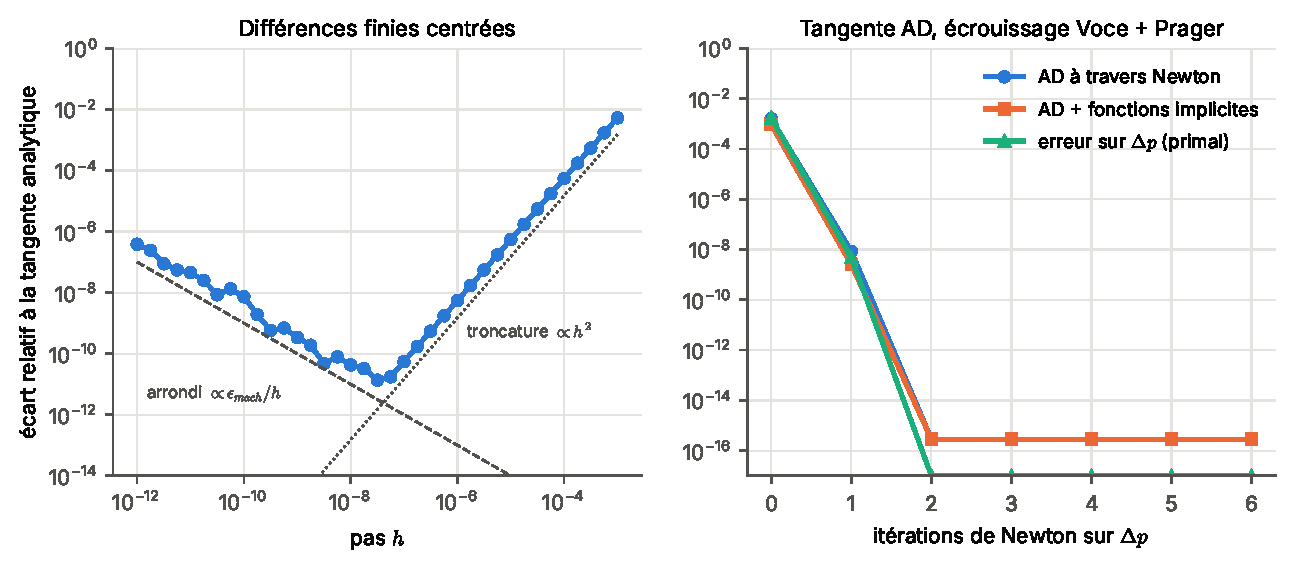
\includegraphics[width=\linewidth]{tangent_accuracy}
\caption{À gauche : erreur des différences finies centrées en fonction du pas $h$. On retrouve la courbe en V de la section~\ref{sec:df}, avec un optimum vers $h^\star\approx3\times10^{-8}$ et une erreur de $1{,}4\times10^{-11}$. À droite : erreur de la tangente AD en fonction du nombre d'itérations du Newton local sur $\Delta p$ (écrouissage Voce + Prager). Les deux modes de dérivation suivent l'erreur sur la solution primale et atteignent l'arrondi en 2 itérations.}\label{fig:tangent}
\end{figure}

\paragraph{Lecture de la figure~\ref{fig:tangent} (gauche).} Le pas optimal prédit est $h^\star\approx\epsilon_{\mathrm{mach}}^{1/3}\times|\eps|\approx6\times10^{-6}\times4\times10^{-3}\approx2\times10^{-8}$ et l'erreur minimale $\epsilon_{\mathrm{mach}}^{2/3}\approx4\times10^{-11}$. Les valeurs mesurées sont $3\times10^{-8}$ et $1{,}4\times10^{-11}$. Les différences finies sont donc une bonne vérification indépendante, mais pas un substitut à l'AD dans un code de production : elles coûtent 12 appels à la loi au lieu d'un, et donnent 5 chiffres de moins.

\paragraph{Lecture de la figure~\ref{fig:tangent} (droite).} L'initialisation $\Delta p^{(0)}$ laisse une erreur relative de $2\times10^{-3}$, qu'une itération réduit à $5\times10^{-9}$ et une deuxième à l'arrondi : c'est la convergence quadratique du Newton local. À 1 itération, la dérivée implicite ($2{,}6\times10^{-9}$) est un peu meilleure que la dérivée à travers les itérations ($8{,}5\times10^{-9}$). Au-delà, les deux sont exactes. Ici l'intérêt de la dérivation implicite n'est donc pas la précision. C'est la \emph{mémoire} en mode inverse et l'indépendance vis-à-vis de l'algorithme de résolution : on pourrait remplacer Newton par une bissection sans changer la dérivée.

\section{Le point matériel : là où la tangente sert}\label{sec:pm}

\subsection{Pilotage mixte}

Un essai de traction « en contrainte » impose $\varepsilon_{11}$ et laisse le matériau libre latéralement : $\sigma_{22}=\sigma_{33}=0$ et les cisaillements sont nuls. Parmi les 6 composantes de $\eps$, on impose donc les composantes $c$ et on cherche les composantes libres $f$ telles que
\begin{equation}
\mathbf{r}(\eps_f) = \sig_f\big(\eps_c,\eps_f\big) = \mathbf{0},
\end{equation}
où $\sig$ est calculée par \code{integrate} à partir de l'état convergé du pas précédent. On résout par Newton : $\mathbf{K}_{ff}\,\delta\eps_f=-\mathbf{r}$, avec $\mathbf{K}$ égal soit à la tangente cohérente (AD), soit à la tangente élastique $\C$. C'est un Newton global « miniature » : il a la même structure que l'équilibre d'un maillage EF, réduit à un seul point.

Paramètres : $E=210$~GPa, $\nu=0{,}3$, $\sigma_y=250$~MPa, $H=1$~GPa et, pour Voce, $Q=150$~MPa, $b=50$. On trace le résidu du second pas, qui fait passer $\varepsilon_{11}$ de $0{,}1\,\%$ (élastique) à $0{,}6\,\%$, un grand incrément plastique.

\begin{figure}[h]
\centering
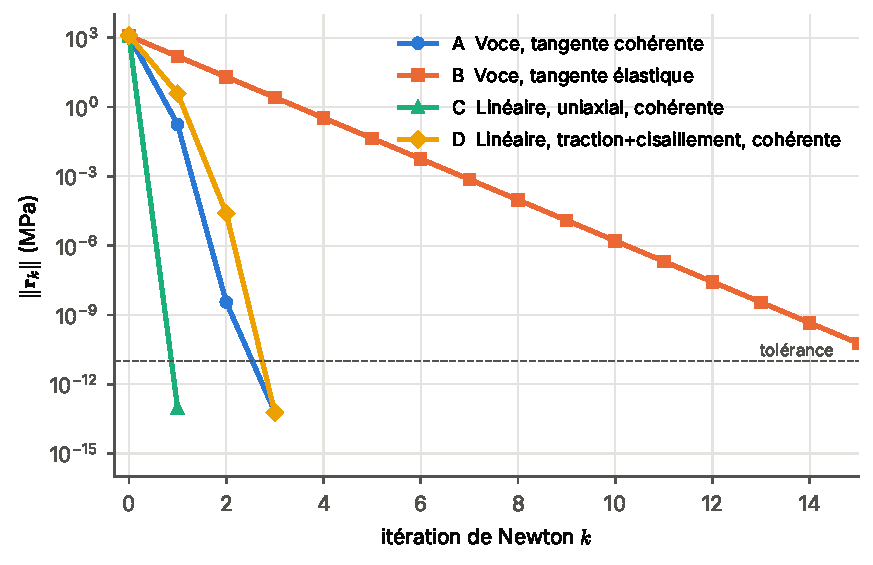
\includegraphics[width=0.78\linewidth]{newton_convergence}
\caption{Norme du résidu (MPa) au cours des itérations de Newton, pour un incrément $\varepsilon_{11}:0{,}1\,\%\to0{,}6\,\%$.}\label{fig:newton}
\end{figure}

\subsection{Résultats}

\begin{table}[h]
\centering
\begin{tabular}{llcc}
\toprule
Cas & Tangente & Itérations & Ordre empirique~\eqref{eq:ordre}\\
\midrule
A : Voce, uniaxial & cohérente & 3 & 2,01\\
B : Voce, uniaxial & élastique & 16 & 1,00 (taux 0,130)\\
C : linéaire, uniaxial & cohérente & 1 & ---\\
D : linéaire, traction + cisaillement & cohérente & 3 & 2,07\\
\bottomrule
\end{tabular}
\caption{Convergence du Newton au point matériel (tolérance $10^{-11}$~MPa).}\label{tab:newton}
\end{table}

\paragraph{Cas A et D : convergence quadratique.} Les résidus successifs du cas A valent $1{,}2\times10^{3}$, $1{,}8\times10^{-1}$, $3{,}6\times10^{-9}$ puis $6\times10^{-14}$. L'exposant double à chaque itération et l'ordre mesuré vaut 2,01. C'est la signature de la tangente cohérente.

\paragraph{Cas B : convergence linéaire.} Avec la tangente élastique, le résidu est multiplié par 0,130 à chaque itération, avec une régularité remarquable : l'ordre vaut 1,00 sur 15 itérations. Ce taux se \emph{prédit}. L'itération de Newton modifiée propage l'erreur par $\mathbf{M}=\mathbf{I}-\mathbf{K}_{e,ff}^{-1}\mathbf{K}_{t,ff}$. Le calcul des valeurs propres de $\mathbf{M}$ au point solution donne 0,1296 pour le mode symétrique $\delta\varepsilon_{22}=\delta\varepsilon_{33}$, et 0,797 pour les modes de cisaillement. Le résidu initial étant purement « latéral », seul le mode symétrique est excité, et on mesure 0,1296. Un chargement de cisaillement aurait convergé au taux 0,8, soit environ 110 itérations pour gagner 11 ordres de grandeur.

\paragraph{Cas C : le piège du sujet.} Avec un écrouissage linéaire en traction proportionnelle, Newton converge en \textbf{une seule} itération. On ne peut donc pas y observer de convergence quadratique. Ce n'est pas un bug : c'est une propriété du problème.

\begin{proposition}
Pour l'écrouissage isotrope (et cinématique) linéaire, en chargement uniaxial proportionnel ($\varepsilon_{22}=\varepsilon_{33}$, état initial de la même forme), la fonction $\varepsilon_{22}\mapsto\sigma_{22}$ calculée par le retour radial est affine par morceaux.
\end{proposition}
\begin{proof}
Toutes les déformations en jeu sont de la forme $a\,\I+b\,\mathbf{D}$ avec $\mathbf{D}=\mathrm{diag}(2,-1,-1)$, et $\epsp_n$, $\X_n$ sont proportionnels à $\mathbf{D}$. Donc $\bs\xi\tri=\beta\,\mathbf{D}$ avec $\beta$ affine en $\varepsilon_{22}$, et sa direction $\n=\pm\mathbf{D}/\|\mathbf{D}\|$ est \emph{constante} par morceaux (selon le signe de $\beta$). Alors $q\tri=\sqrt{3/2}\,\|\mathbf{D}\|\,|\beta|$ est affine par morceaux, $\Delta p=(q\tri-R(p_n))/(3\mu+h)$ l'est aussi, et $\sig_{n+1}=\sig\tri-2\mu\Delta p\N$ est affine par morceaux en $\varepsilon_{22}$. Newton résout exactement un problème affine en une itération, dès que l'itéré est dans le bon morceau (élastique ou plastique).
\end{proof}

La non-linéarité qui rend la tangente cohérente indispensable a deux sources : la courbure de $R(p)$ (cas A) et la \emph{rotation} de la direction d'écoulement $\n$ (cas D, où le rapport cisaillement/traction change au cours du pas). Dans un vrai calcul de structure, les deux sont presque toujours présentes. Pour \emph{démontrer} la convergence quadratique sur un point matériel, il faut donc choisir l'un de ces deux ingrédients.

\subsection{Chargement cyclique et hystérésis}

On impose $\varepsilon_{11}$ en triangle d'amplitude $\pm0{,}8\,\%$ pendant 3 cycles, avec contraintes latérales nulles, pour trois écrouissages (figure~\ref{fig:hyst}).

\begin{figure}[h]
\centering
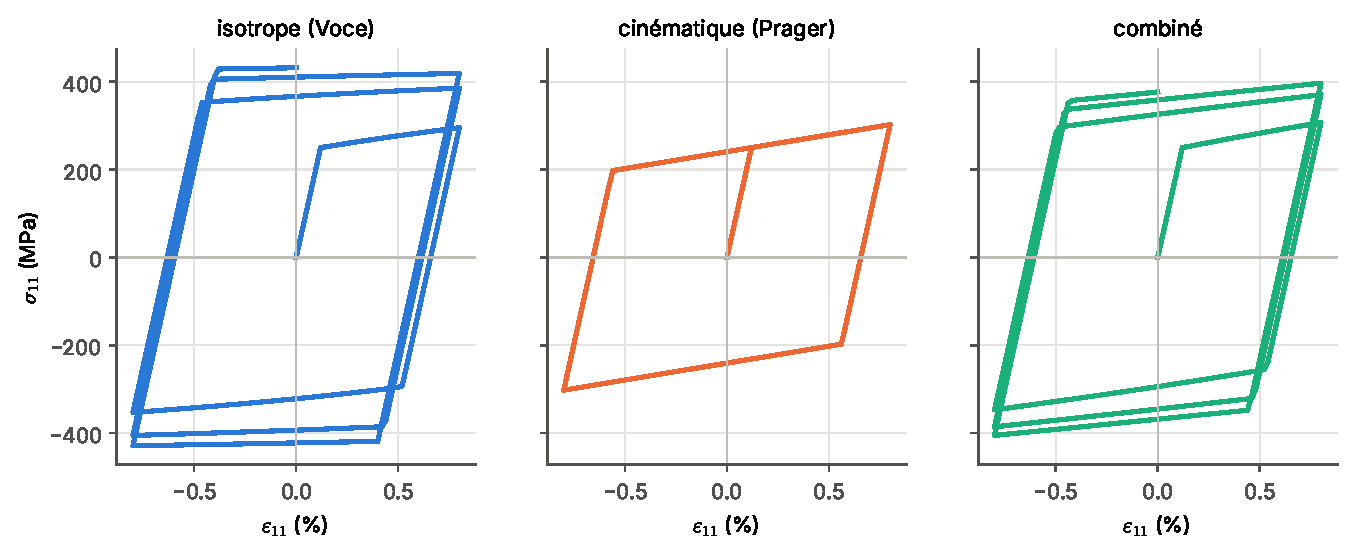
\includegraphics[width=\linewidth]{hysteresis}
\caption{Boucles contrainte--déformation en traction--compression cyclique (3 cycles, $\pm0{,}8\,\%$). Isotrope : $H=0{,}5$~GPa, $Q=150$~MPa, $b=50$. Cinématique : $C=8$~GPa. Combiné : $H=0{,}5$~GPa, $Q=100$~MPa, $b=50$, $C=4$~GPa.}\label{fig:hyst}
\end{figure}

\begin{itemize}
  \item \textbf{Isotrope.} Le domaine d'élasticité grossit à chaque passage plastique. Le pic de traction passe de 295~MPa au premier cycle à 419~MPa au troisième, et le pic de compression de $-353$ à $-429$~MPa. En inversion de charge, la plastification ne commence qu'à $-\sigma_{\text{pic}}$ : il n'y a \emph{pas} d'effet Bauschinger, ce qui est contraire à l'expérience sur les métaux.
  \item \textbf{Cinématique.} Le domaine garde sa taille ($2\sigma_y=500$~MPa) et se translate. Après une traction jusqu'à $+302{,}5$~MPa, la plastification inverse commence vers $302{,}5-500$, soit $-197{,}5$~MPa : c'est l'effet Bauschinger. La boucle est stabilisée dès le premier cycle et se superpose ensuite à elle-même.
  \item \textbf{Combiné.} Les deux mécanismes coexistent : on voit un effet Bauschinger et une boucle qui grossit en tendant vers une saturation, au rythme de $R(p)$ (pics de traction de 307 puis 371 et 397~MPa, de compression de $-347$ à $-406$~MPa). C'est le comportement qualitatif d'un acier, que les lois de type Chaboche affinent avec un écrouissage cinématique non linéaire.
\end{itemize}
Le Newton converge en au plus 3 itérations à chaque pas, y compris aux inversions de charge, où le pas passe du plastique à l'élastique.

\section{Intégration par lots et performances}\label{sec:perf}

\subsection{Vectorisation}

Dans un code EF, la loi est appelée sur tous les points de Gauss du maillage à chaque itération, et ces appels sont indépendants. La fonction écrite pour \emph{un} point se vectorise en une ligne :
\begin{lstlisting}
batched = jax.jit(jax.vmap(integrate, in_axes=(0, 0, None)))   # params partages
sigma, state = batched(eps[N,6], State(eps_p[N,6], p[N], alpha[N,6]), params)
\end{lstlisting}
Comme les deux branches de chaque \code{where} sont calculées, le coût d'un point ne dépend \emph{pas} de son état. Il n'y a ni divergence de branches sur GPU, ni masque vectoriel coûteux sur CPU. Dans nos données, 99,8\,\% des points plastifient, mais un lot entièrement élastique coûterait pareil. Le corollaire est qu'il est inutile d'espérer gagner du temps sur les points élastiques.

\subsection{Modèle de performance}

\begin{rappel}{modèle roofline}
Le temps d'un noyau est borné inférieurement par $\max\big(W/F,\ Q/B\big)$, où $W$ est le nombre d'opérations flottantes, $F$ le débit crête de calcul, $Q$ le volume de données échangé avec la mémoire et $B$ la bande passante~\cite{williams2009}. Le rapport $I=W/Q$ (flop/octet) est l'\emph{intensité arithmétique}. Si $I<F/B$ (le « point d'équilibre » de la machine), le noyau est limité par la mémoire, sinon par le calcul.
\end{rappel}

\paragraph{Comptage pour un point de Gauss.}
\begin{itemize}[nosep]
  \item \emph{Volume minimal} : lire $\eps,\epsp,p,\X$ (19 nombres) et écrire $\sig,\epsp,p,\X$ (19 nombres), soit $Q_{\min}=38$ mots, c'est-à-dire 304~octets en FP64 et 152 en FP32.
  \item \emph{Opérations} : XLA en compte 228 (\code{cost\_analysis}). En faisant varier le nombre d'itérations de Newton, on constate que ce compte n'inclut le corps de la boucle qu'une fois. L'estimation réelle est d'environ 300~flops et une dizaine d'exponentielles par point.
  \item \emph{Intensité} : $I\approx1$~flop/octet en FP64. C'est très faible : un CPU moderne a un point d'équilibre de 5 à 20~flop/octet. Le noyau est donc \textbf{limité par la mémoire} sur CPU.
\end{itemize}

\paragraph{Ce que fait réellement XLA.} L'examen du code compilé (\code{compiled.as\_text()}) montre que XLA ne produit pas \emph{un} noyau. Il en produit 12 fusions, plus une boucle \code{while} pour le Newton. Des intermédiaires de taille $N\times6$, comme $\bs\xi\tri$, sont donc écrits en mémoire puis relus par plusieurs consommateurs. Le trafic estimé par XLA est de 1072~octets par point en FP64, soit \textbf{3,5 fois le minimum}. Dérouler la boucle (\code{unroll=True}) ne change rien (1200~octets, débit identique à 5\,\% près). Pour atteindre le minimum il faudrait un noyau écrit à la main, par exemple en Pallas, Numba ou C++/CUDA, qui fasse tout en registres. C'est une piste d'optimisation identifiée, mais non réalisée ici.

\subsection{Mesures sur CPU}

Configuration : NumPy vectorisé et JAX CPU, FP64 et FP32, $N$ de $10^2$ à $3\times10^6$. On ne va pas jusqu'à $10^7$ : la version NumPy, avec ses temporaires, dépasse les 7~Go de la machine virtuelle. Chaque point de mesure est la médiane d'au moins 3 appels et d'au moins 0,3~s de mesure. La compilation est mesurée à part.

\begin{figure}[h]
\centering
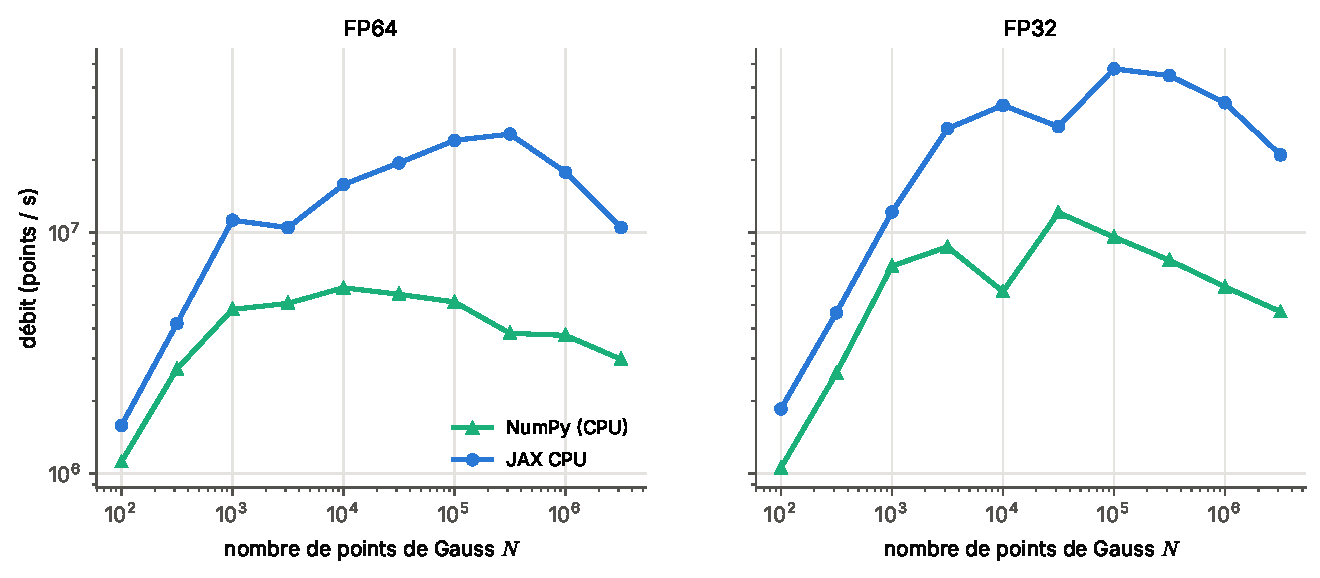
\includegraphics[width=\linewidth]{bench_cpu_throughput}
\caption{Débit (points de Gauss par seconde) en fonction de $N$, machine virtuelle 2 cœurs. Écrouissage Voce + Prager, 4 itérations de Newton local.}\label{fig:bench-thr}
\end{figure}

\begin{figure}[h]
\centering
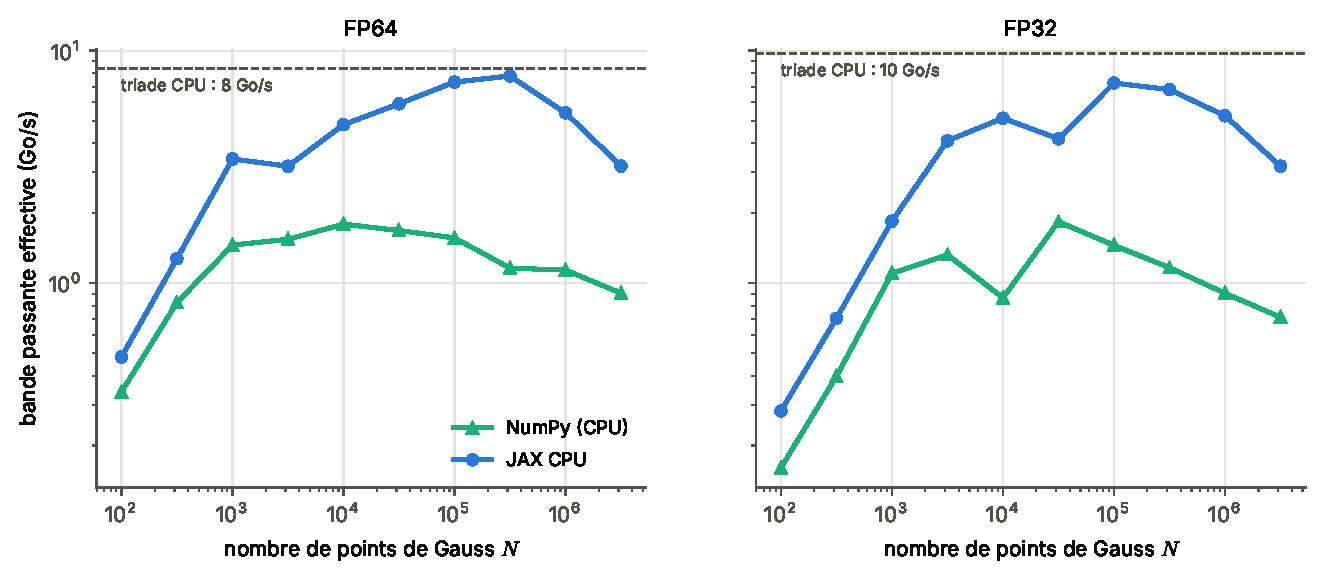
\includegraphics[width=\linewidth]{bench_cpu_bandwidth}
\caption{Bande passante effective calculée sur le volume \emph{minimal} (304~o/point en FP64), comparée à la bande passante d'une triade $z=ax+y$ sur de grands tableaux (mémoire principale).}\label{fig:bench-bw}
\end{figure}

\begin{table}[h]
\centering
\begin{tabular}{lcccc}
\toprule
 & \multicolumn{2}{c}{FP64} & \multicolumn{2}{c}{FP32}\\
\cmidrule(lr){2-3}\cmidrule(lr){4-5}
 & meilleur débit & à $N=3\times10^6$ & meilleur débit & à $N=3\times10^6$\\
\midrule
NumPy & $5{,}9\times10^6$ & $3{,}0\times10^6$ & $1{,}2\times10^7$ & $4{,}7\times10^6$\\
JAX CPU & $2{,}6\times10^7$ & $1{,}05\times10^7$ & $4{,}8\times10^7$ & $2{,}1\times10^7$\\
rapport JAX / NumPy & $4{,}3$ & $3{,}5$ & $4{,}0$ & $4{,}5$\\
\bottomrule
\end{tabular}
\caption{Débits mesurés (points/s). Temps de compilation JAX : 0,16 à 0,23~s, indépendant de $N$.}\label{tab:bench}
\end{table}

\paragraph{Lecture des résultats.}
\begin{enumerate}
  \item \textbf{Petits lots ($N\lesssim10^3$).} Le temps est dominé par le coût fixe d'un appel, environ 60~µs pour JAX : dispatch Python et lancement du noyau. Le débit croît alors linéairement avec $N$. Dans un code EF, cela plaide pour un appel par \emph{maillage} et non par élément.
  \item \textbf{Lots moyens ($10^4$ à $3\times10^5$).} Les données (30 à 100~Mo, auxquels s'ajoutent les intermédiaires) tiennent dans le grand cache L3 de la machine hôte (260~Mo). JAX atteint $2{,}6\times10^7$ points/s en FP64, soit 4,3 fois NumPy. Le gain vient de la fusion : NumPy matérialise chaque opération dans un temporaire de taille $N$, alors que XLA en élimine la plupart.
  \item \textbf{Grands lots ($N\ge10^6$).} Les données sortent du cache et le débit chute à $1{,}05\times10^7$ points/s. En volume \emph{réel} (1072~o/point), cela représente 11~Go/s, du même ordre que la bande passante de la triade (8,4~Go/s), une partie des intermédiaires restant en cache. Le noyau est donc bien limité par la mémoire. Le facteur 3,5 de trafic superflu se paie directement en temps.
  \item \textbf{FP32 contre FP64.} En FP32, le débit est 1,8 à 2 fois plus élevé, exactement le rapport des volumes de données. C'est une autre confirmation que le noyau est limité par la mémoire et non par le calcul.
  \item \textbf{Compilation.} 0,2~s par forme de tableau. C'est négligeable devant un calcul, mais \code{jit} recompile pour chaque nouveau $N$. Un code EF doit donc garder des formes fixes, en complétant les lots par du remplissage si nécessaire.
\end{enumerate}

\subsection{Mesures sur GPU : RTX~2050 portable}\label{sec:gpu}

\paragraph{Machine et méthode.} Portable Lenovo LOQ : processeur i5-12450HX (8 cœurs, 12 threads), carte NVIDIA GeForce RTX~2050 (architecture Ampere, 4~Go de GDDR6 sur un bus de 64~bits, PCIe~3.0~x8), pilote 595.99, JAX~0.12 avec CUDA~13. Les mesures sont faites avec le kit du dossier \code{gpu/} (annexe~\ref{app:repo}). Avant toute mesure, deux vérifications :
\begin{itemize}[nosep]
  \item les 77 tests passent sur la machine ;
  \item le GPU donne les mêmes contraintes que NumPy, avec un écart relatif de $1{,}1\times10^{-16}$ en FP64 et $1{,}3\times10^{-7}$ en FP32 (arrondi de la simple précision).
\end{itemize}

\paragraph{Les plafonds de la machine.} Le script \code{check\_gpu.py} mesure les limites matérielles qui servent de référence (tableau~\ref{tab:plafonds}).

\begin{table}[h]
\centering
\begin{tabular}{lcc}
\toprule
Grandeur & Mesurée & Théorique\\
\midrule
PCIe hôte $\to$ GPU & 4,9~Go/s & 7,9~Go/s\\
PCIe GPU $\to$ hôte & 2,2~Go/s & 7,9~Go/s\\
bande passante mémoire GPU (triade) & 91--94~Go/s & 112~Go/s\\
bande passante mémoire CPU (triade) & 20--21~Go/s & ---\\
calcul GPU FP32 (produit de matrices) & 5475~GFLOP/s & 6020~GFLOP/s\\
calcul GPU FP64 (produit de matrices) & 106~GFLOP/s & 94~GFLOP/s\\
rapport FP64 / FP32 & 1/52 & 1/64\\
latence d'un appel JAX & 31~µs & ---\\
\bottomrule
\end{tabular}
\caption{Plafonds mesurés sur la machine.}\label{tab:plafonds}
\end{table}

\begin{piege}{le FP64 sur GPU grand public}
Une carte « gaming » n'a qu'une unité FP64 pour 64 unités FP32. Les cartes de calcul (A100, H100) ont un rapport de 1/2. La mesure confirme l'ordre de grandeur : 106~GFLOP/s en FP64 contre 5475 en FP32, soit un rapport de 1/52. En FP64, la RTX~2050 calcule donc moins vite que le processeur du même portable.
\end{piege}

\begin{figure}[h]
\centering
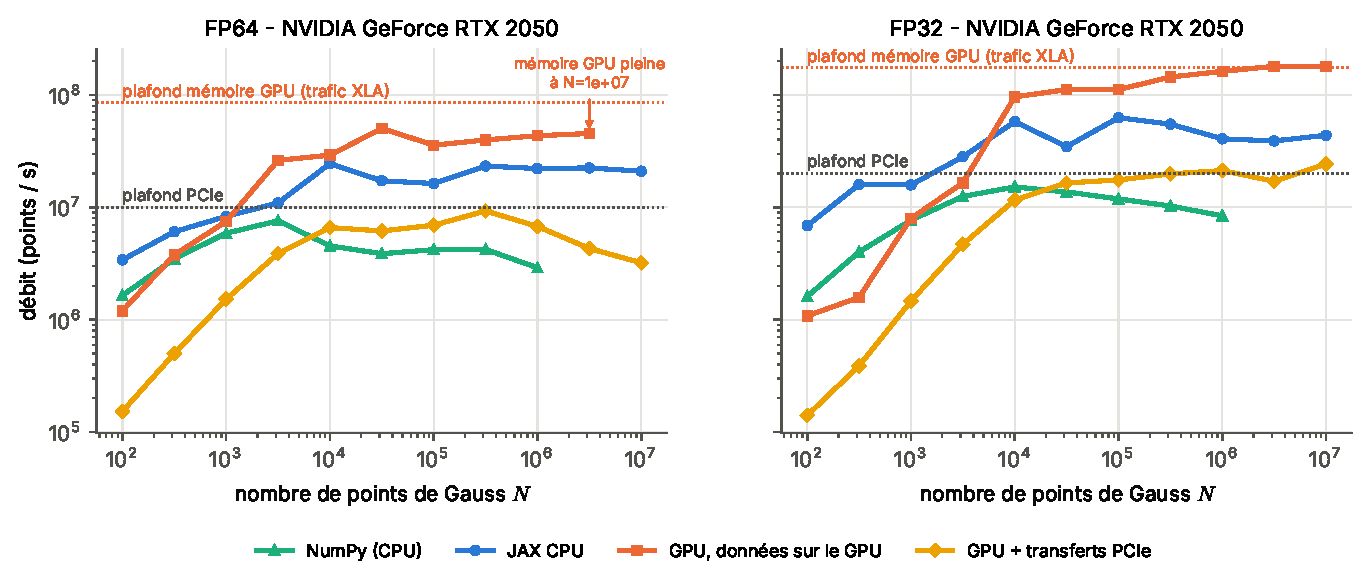
\includegraphics[width=\linewidth]{gpu_throughput_izanami-LOQ-15IAX9}
\caption{Débit mesuré en fonction de $N$ sur la machine équipée de la RTX~2050. Les pointillés sont les plafonds calculés à partir des mesures du tableau~\ref{tab:plafonds}. Plafond mémoire GPU : triade divisée par le trafic réel d'XLA (1072~o/point en FP64, 536 en FP32). Plafond PCIe : envoi de 19 nombres et retour de 19 nombres par point, aux débits mesurés.}\label{fig:gpu-thr}
\end{figure}

\begin{figure}[h]
\centering
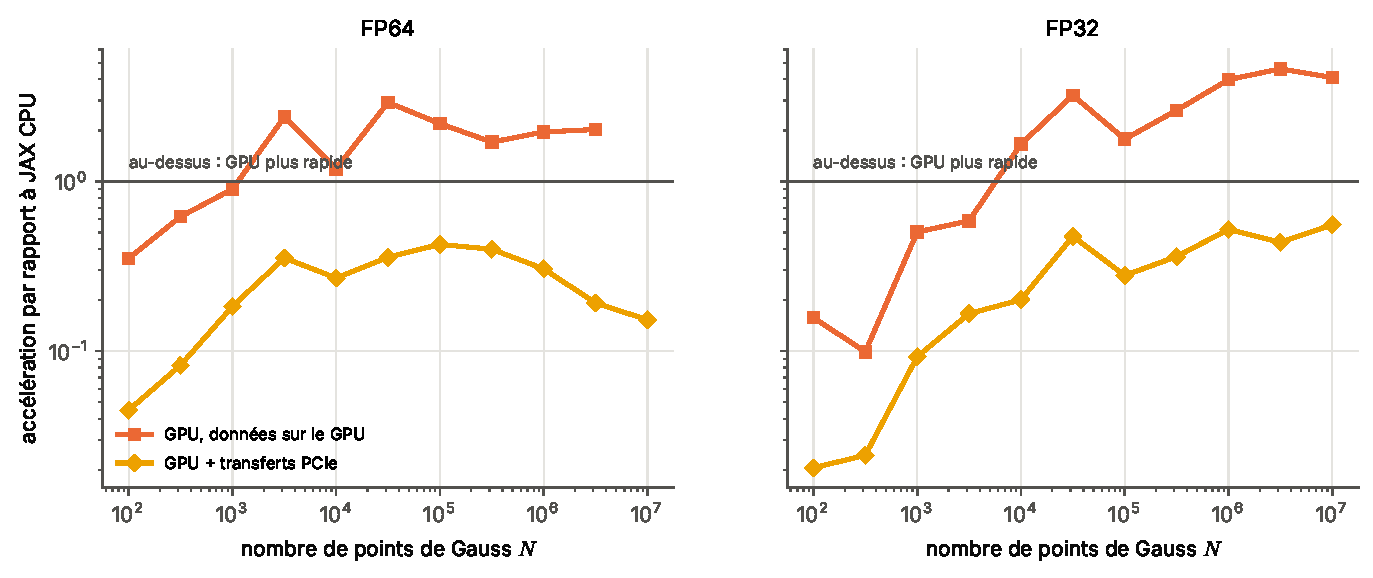
\includegraphics[width=\linewidth]{gpu_speedup_izanami-LOQ-15IAX9}
\caption{Accélération par rapport à JAX CPU (12 threads). Au-dessus de 1, le GPU est plus rapide.}\label{fig:gpu-speedup}
\end{figure}

\begin{table}[h]
\centering
\begin{tabular}{lcccc}
\toprule
 & NumPy & JAX CPU & GPU, données résidentes & GPU + transferts\\
\midrule
FP64 & $2{,}9\times10^6$ & $2{,}2\times10^7$ & $4{,}3\times10^7$ ($\times2{,}0$) & $6{,}8\times10^6$ ($\times0{,}31$)\\
FP32 & $8{,}4\times10^6$ & $4{,}1\times10^7$ & $1{,}6\times10^8$ ($\times4{,}0$) & $2{,}1\times10^7$ ($\times0{,}52$)\\
\bottomrule
\end{tabular}
\caption{Débits mesurés (points/s) à $N=10^6$. Entre parenthèses : l'accélération par rapport à JAX CPU.}\label{tab:gpu}
\end{table}

\paragraph{Lecture des résultats.}
\begin{enumerate}
  \item \textbf{Les plafonds se vérifient presque au point près.}
  \begin{itemize}[nosep]
    \item En FP32, le GPU avec données résidentes atteint $1{,}79\times10^8$ points/s pour un plafond mémoire de $1{,}76\times10^8$ : il est exactement \textbf{limité par la bande passante}, avec le trafic réel d'XLA (3,5 fois le minimum, section~\ref{sec:perf}).
    \item Sur CPU, JAX en FP64 atteint $2{,}2\times10^7$ points/s pour un plafond de $21{,}4\ \text{Go/s} / 1072\ \text{o} = 2{,}0\times10^7$ : également limité par la mémoire.
    \item La découpe du noyau en 12 fusions par XLA coûte donc le même facteur 3,5 sur CPU et sur GPU.
  \end{itemize}
  \item \textbf{En FP64, le GPU est limité par ses unités de calcul.} Il plafonne à $4{,}5\times10^7$ points/s, soit seulement 53\,\% de son plafond mémoire. La division, la racine carrée et l'exponentielle de Voce en FP64 coûtent chacune des dizaines d'opérations sur des unités 52 fois moins nombreuses. C'est pourquoi le rapport FP32/FP64 sur GPU vaut 4 : ce n'est ni 2 (rapport des volumes de données, comme sur CPU), ni 52 (rapport des unités de calcul).
  \item \textbf{Avec données résidentes, le GPU gagne}, d'un facteur 2 en FP64 et de 4 à 4,6 en FP32 pour les grands lots. Le point de bascule est à $N\approx3\times10^3$ en FP64 et $10^4$ en FP32. En dessous de $10^3$ points, le GPU est plus lent : le coût fixe d'un lancement (31~µs pour un appel vide, environ 80~µs pour le noyau) domine.
  \item \textbf{Avec les transferts, le GPU perd toujours.} Il atteint au mieux 0,43 fois la vitesse du CPU en FP64 et 0,56 fois en FP32. Le plafond PCIe calculé avec les débits mesurés,
  \[
  \Big(\tfrac{152\ \text{o}}{4{,}86\ \text{Go/s}}+\tfrac{152\ \text{o}}{2{,}20\ \text{Go/s}}\Big)^{-1} = 1{,}0\times10^7\ \text{points/s en FP64},
  \]
  est atteint à 93\,\% ($9{,}3\times10^6$). Il reste inférieur au débit du CPU seul ($2{,}2\times10^7$).
  \item \textbf{Où passe le temps} (figure~\ref{fig:gpu-bd}) : à $N=10^7$, le calcul ne représente que 11 à 13\,\% du temps. Le retour des résultats en prend 51 à 64\,\% et l'envoi 25 à 36\,\%. Le retour est plus lent que l'envoi parce que la mémoire de l'hôte n'est pas « verrouillée » (\emph{pageable}) : le pilote doit faire une copie intermédiaire.
  \item \textbf{La mémoire de 4~Go limite la taille des lots.} À $N=10^7$ en FP64, la version « données résidentes » échoue : XLA demande 3,04~Go d'arguments pour une limite de 2,97~Go. La version avec transferts fonctionne grâce au découpage en blocs de $2^{20}$ points.
\end{enumerate}

\begin{figure}[h]
\centering
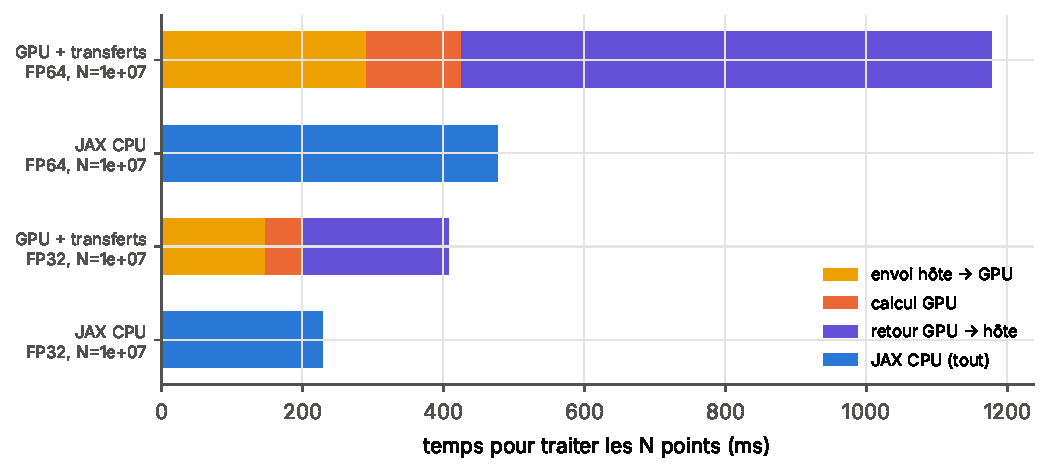
\includegraphics[width=0.85\linewidth]{gpu_breakdown_izanami-LOQ-15IAX9}
\caption{Décomposition du temps à $N=10^7$ : envoi, calcul et retour (chaque étape synchronisée), comparés au temps total de JAX CPU.}\label{fig:gpu-bd}
\end{figure}

\paragraph{Une limite de la mesure.} Aux plus grands $N$ en FP64, le débit de bout en bout avec transferts chute ($3{,}2\times10^6$ points/s à $N=10^7$). Pourtant, la somme des trois étapes mesurées séparément ne fait que 1,18~s, contre 3,1~s de bout en bout. L'écart vient d'un coût côté hôte : les 1,5~Go de tableaux de sortie étaient alloués à chaque répétition, et le système doit fournir ces pages mémoire au premier accès. Le kit a été corrigé pour allouer les sorties une seule fois. Même avec la somme des étapes ($8{,}5\times10^6$ points/s), le GPU reste 2,5 fois plus lent que le CPU : la conclusion ne change pas.

\paragraph{Comparaison avec le modèle a priori.} Avant de disposer de la machine, un modèle roofline avait été construit à partir des caractéristiques constructeur (tableau~\ref{tab:modele}).

\begin{table}[h]
\centering
\small
\begin{tabular}{lcc}
\toprule
Quantité & Prédiction & Mesure\\
\midrule
GPU résident, FP32 & $1{,}7$ à $5{,}9\times10^8$ & $1{,}8\times10^8$ (= borne XLA)\\
GPU résident, FP64 & $0{,}8$ à $1{,}9\times10^8$ & $4{,}5\times10^7$\\
GPU + transferts, FP64 & $\le2\times10^7$ (6~Go/s) & $9{,}3\times10^6$ (retour 2,2~Go/s)\\
GPU rentable avec transferts ? & non & non\\
\bottomrule
\end{tabular}
\caption{Modèle a priori contre mesures (points/s).}\label{tab:modele}
\end{table}

Le modèle avait raison sur la conclusion principale, et sur le FP32. Il était trop optimiste de 2 à 4 en FP64, car il sous-estimait le coût des fonctions spéciales en double précision sur ces unités. Il était aussi trop optimiste d'un facteur 2 sur le PCIe, car le retour vers l'hôte est deux fois plus lent que l'envoi.

\subsection{Conséquences pour une interface code\_aster--JAXMat}

\begin{itemize}
  \item \textbf{Transférer tout l'état à chaque appel n'est pas rentable}, quel que soit $N$. Les mesures le confirment.
  \item \textbf{Garder les variables internes sur le GPU} entre les itérations de Newton change la donne. L'état ($\epsp$, $p$, $\X$) ne voyage plus : seuls $\eps$ (6 nombres) et $\sig$ (6 nombres) circulent, soit 96~o/point en FP64 au lieu de 304. Le plafond PCIe passe alors à $3{,}2\times10^7$ points/s, au-dessus du CPU ($2{,}2\times10^7$). C'est l'expérience à faire en priorité.
  \item \textbf{La tangente ne doit pas revenir sur le CPU.} Avec 36 nombres de plus par point, le plafond PCIe retombe à $6\times10^6$ points/s. Pour profiter du GPU avec un Newton complet, l'assemblage de $\mathbf{K}$ doit lui aussi se faire sur le GPU.
  \item \textbf{La mémoire hôte verrouillée} (\code{memory\_kind="pinned\_host"} dans JAX) devrait rapprocher le retour des 6 à 7~Go/s du bus PCIe.
  \item \textbf{FP32 ou précision mixte ?} Le gain du FP32 sur GPU (facteur 4) est tentant, mais une tangente en simple précision limite la précision de la convergence de Newton (section~\ref{sec:maths}). Une piste est la précision mixte : la loi en FP32, le résidu d'équilibre en FP64.
\end{itemize}

\subsection{Reproduire les mesures}\label{sec:protocole-gpu}

Le dossier \code{gpu/} contient un kit autonome, documenté dans \code{gpu/README\_GPU.md} :
\begin{lstlisting}[language=bash]
bash gpu/setup_gpu.sh            # venv + jax[cuda12/13] selon le pilote (une fois)
source .venv-gpu/bin/activate
bash gpu/run_all.sh              # tests, diagnostic, benchmark, figures, archive
\end{lstlisting}
Le benchmark vérifie d'abord l'exactitude du GPU contre NumPy. Il traite les grands lots par blocs de taille fixe, pour éviter de manquer de mémoire et de recompiler, et mesure séparément l'envoi, le calcul et le retour. Il désactive aussi la pré-allocation de JAX (\code{XLA\_PYTHON\_CLIENT\_PREALLOCATE=false}).

\section{Bonus : hyperélasticité et potentiel neuronal}\label{sec:hyper}

\subsection{Rappels de grandes déformations}

On quitte l'hypothèse des petites perturbations. Le mouvement $\mathbf{x}=\bs\varphi(\mathbf{X})$ envoie la configuration de référence sur la configuration actuelle. On définit le gradient de la transformation $\F$, la variation de volume $J$, le tenseur de Cauchy--Green droit $\mathbf{C}$ et ses invariants :
\begin{align*}
&\F = \frac{\partial\mathbf{x}}{\partial\mathbf{X}}, && J=\det\F>0,\\
&\mathbf{C}=\F^T\F \ \text{(Cauchy--Green droit)}, && I_1=\tr\mathbf{C},\quad I_2=\tfrac12\big[(\tr\mathbf{C})^2-\tr(\mathbf{C}^2)\big],\quad I_3=\det\mathbf{C}=J^2.
\end{align*}
$\mathbf{C}$ ne dépend pas d'une rotation superposée ($\F\to\mathbf{Q}\F$ laisse $\mathbf{C}$ invariant). Il mesure donc la déformation « pure ». Pour un étirement diagonal $\F=\mathrm{diag}(\lambda_1,\lambda_2,\lambda_3)$, on a $I_1=\sum\lambda_i^2$ et $I_2=\sum_{i<j}\lambda_i^2\lambda_j^2$.

\paragraph{Hyperélasticité.} Un matériau est hyperélastique s'il existe une énergie libre $\psi(\F)$ par unité de volume de référence telle que la contrainte nominale (premier tenseur de Piola--Kirchhoff) soit
\begin{equation}
\Pk = \frac{\partial\psi}{\partial\F},\qquad \sig = J^{-1}\Pk\F^T,\qquad \mathbb{A}=\frac{\partial^2\psi}{\partial\F\,\partial\F}.
\end{equation}
\emph{Objectivité} : $\psi(\mathbf{Q}\F)=\psi(\F)$ pour toute rotation $\mathbf{Q}$, ce qui impose que $\psi$ ne dépende que de $\mathbf{C}$. \emph{Isotropie} : $\psi$ ne dépend alors que de $(I_1,I_2,J)$. $\mathbb{A}$ a toujours la symétrie majeure, puisque c'est une hessienne.

\subsection{Neo-Hooke compressible : la dérivation devient inutile}

\begin{equation}
\psi(\F) = \frac\mu2\big(I_1-3-2\ln J\big)+\frac\lambda2(\ln J)^2.
\end{equation}
Avec $\partial I_1/\partial\F=2\F$ et $\partial J/\partial\F=J\F^{-T}$, la dérivation à la main donne
\begin{align}
\Pk &= \mu(\F-\F^{-T})+\lambda\ln J\,\F^{-T},\\
\mathbb{A}_{iJkL} &= \mu\,\delta_{ik}\delta_{JL} + (\mu-\lambda\ln J)\,F^{-1}_{Li}F^{-1}_{Jk} + \lambda\,F^{-1}_{Ji}F^{-1}_{Lk}.
\end{align}
Avec JAX, on écrit seulement $\psi$ :
\begin{lstlisting}
def psi_neo_hooke(F, mu, lam):
    I1 = jnp.sum(F * F); lnJ = jnp.log(jnp.linalg.det(F))
    return 0.5 * mu * (I1 - 3.0 - 2.0 * lnJ) + 0.5 * lam * lnJ**2

P = jax.grad(psi_neo_hooke)(F, mu, lam)        # 3x3
A = jax.hessian(psi_neo_hooke)(F, mu, lam)     # 3x3x3x3
\end{lstlisting}
Sur des $\F$ aléatoires, l'écart avec les formules analytiques est de $2\times10^{-16}$ pour $\Pk$ et de $10^{-15}$ pour $\mathbb{A}$. Les tests vérifient aussi $\Pk(\I)=\mathbf{0}$, la symétrie majeure de $\mathbb{A}$ et l'objectivité $\Pk(\mathbf{Q}\F)=\mathbf{Q}\Pk(\F)$. Ici $\F$ n'a pas de symétrie, donc dériver par rapport à la matrice $3\times3$ est correct : le piège de la section~\ref{sec:jax} ne concerne que les arguments symétriques.

\subsection{Incompressibilité et essais homogènes}

Le caoutchouc est quasi incompressible ($K/\mu\sim10^3$). On impose $J=1$ par un multiplicateur de Lagrange $p$, la pression :
\[
\tilde\psi = \psi(I_1,I_2)-p(J-1)\quad\Longrightarrow\quad \Pk = 2\psi_1\F + 2\psi_2\big(I_1\F-\F\mathbf{C}\big) - p\,\F^{-T},\qquad \psi_i=\frac{\partial\psi}{\partial I_i}.
\]
La pression n'est pas donnée par la loi : elle est fixée par les conditions aux limites. Pour les trois essais de Treloar, on la détermine par la condition de bord libre.

\paragraph{Traction uniaxiale (UT).} $\F=\mathrm{diag}(\lambda,\lambda^{-1/2},\lambda^{-1/2})$. La condition $P_{22}=0$ donne $p=2\psi_1\lambda^{-1}+2\psi_2(I_1\lambda^{-1}-\lambda^{-2})$. En reportant dans $P_{11}$ et en utilisant $I_1=\lambda^2+2\lambda^{-1}$ :
\begin{equation}
P_{\mathrm{UT}} = 2\big(\lambda-\lambda^{-2}\big)\big(\psi_1+\lambda^{-1}\psi_2\big).
\end{equation}
\paragraph{Équibiaxiale (ET)} ($\F=\mathrm{diag}(\lambda,\lambda,\lambda^{-2})$) et \textbf{cisaillement pur (PS)} ($\F=\mathrm{diag}(\lambda,1,\lambda^{-1})$). Le même calcul donne
\begin{equation}
P_{\mathrm{ET}} = 2\big(\lambda-\lambda^{-5}\big)\big(\psi_1+\lambda^2\psi_2\big),\qquad P_{\mathrm{PS}} = 2\big(\lambda-\lambda^{-3}\big)\big(\psi_1+\psi_2\big).
\end{equation}
Dans le code, $\psi_1$ et $\psi_2$ sont obtenues par \code{jax.grad} du potentiel, \emph{quel qu'il soit} : analytique ou réseau de neurones.

\subsection{Potentiels étudiés}

\begin{center}
\begin{tabular}{lll}
\toprule
Modèle & $\psi(I_1,I_2)$ & paramètres\\
\midrule
Neo-Hooke & $C_{10}(I_1-3)$ & 1\\
Mooney--Rivlin & $C_{10}(I_1-3)+C_{01}(I_2-3)$ & 2\\
Yeoh~\cite{yeoh1993} & $C_{10}(I_1-3)+C_{20}(I_1-3)^2+C_{30}(I_1-3)^3$ & 3\\
ICNN & réseau convexe en entrée, ci-dessous & 230\\
\bottomrule
\end{tabular}
\end{center}

\begin{rappel}{polyconvexité}
Pour qu'un problème d'hyperélasticité ait une solution (théorème de Ball~\cite{ball1977}), on demande que $\psi$ soit \emph{polyconvexe} : convexe en $(\F,\operatorname{cof}\F,\det\F)$. Or $I_1=\|\F\|^2$ est convexe en $\F$ et $I_2=\|\operatorname{cof}\F\|^2$ est convexe en $\operatorname{cof}\F$. Par la règle de composition des fonctions convexes, \emph{si $h(I_1,I_2)$ est convexe et croissante en chacun de ses arguments, alors $\psi=h(I_1,I_2)$ est polyconvexe}.
\end{rappel}

\paragraph{Réseau convexe en entrée (ICNN).} D'après~\cite{amos2017}, on construit $h$ convexe et croissante par construction. Avec $\mathbf{x}=(I_1-3,\,I_2-3)/10$ :
\begin{align*}
\mathbf{h}_1 &= \mathrm{sp}\big(W_1^{+}\mathbf{x}+\mathbf{b}_1\big),\\
\mathbf{z}_2 &= W_2^{+}\mathbf{h}_1+U_2^{+}\mathbf{x}+\mathbf{b}_2,\qquad \mathbf{h}_2=\big(\mathrm{sp}(\mathbf{z}_2^{(1)}),\ \mathrm{sp}(\mathbf{z}_2^{(2)})^2\big),\\
\psi_\theta &= \mathbf{a}^{+}\cdot\mathbf{h}_2+\mathbf{c}^{+}\cdot\mathbf{x}\ -\ (\text{même expression en }\mathbf{x}=\mathbf{0}),
\end{align*}
où $\mathrm{sp}(z)=\ln(1+e^z)$ (softplus) et l'exposant $+$ désigne des poids rendus positifs par une reparamétrisation softplus. Toutes les activations sont convexes et croissantes et tous les poids qui s'appliquent à des fonctions convexes sont positifs, donc $\psi_\theta$ est convexe et croissante en $\mathbf{x}$. La moitié des neurones en $\mathrm{sp}^2$ permet une croissance superlinéaire, nécessaire pour reproduire le raidissement aux grandes élongations. La soustraction de la valeur en $\mathbf{x}=\mathbf{0}$ garantit une énergie nulle dans l'état de référence. La contrainte y est automatiquement nulle, grâce aux facteurs $(\lambda-\lambda^{-k})$. Avec une largeur de 12, le réseau a 230 paramètres. Le test \code{test\_icnn\_convex\_and\_monotone} vérifie $\psi_1,\psi_2\ge0$ et le caractère semi-défini positif de la hessienne en 20 points aléatoires.

\subsection{Données et identification}

Les données de Treloar~\cite{treloar1944} (caoutchouc naturel vulcanisé) comportent 25 points en traction uniaxiale ($\lambda\le7{,}6$), 14 en équibiaxiale ($\lambda\le4{,}4$) et 14 en cisaillement pur ($\lambda\le4{,}9$). Elles ont été numérisées dans un dépôt public\footnote{Fichier \code{demos/\_data/Treloar\_rubber.csv} du dépôt GitHub \code{jaxmat}, recopié dans \code{data/treloar.csv}.}. La fonction coût est la moyenne, sur les essais, de l'erreur quadratique normalisée
\begin{equation}
\mathcal{L}=\frac{1}{n_e}\sum_{e}\frac{\overline{(P_{\mathrm{mod}}-P_{\exp})^2}}{\overline{P_{\exp}^2}},
\end{equation}
pour que chaque essai pèse autant quelle que soit l'échelle de ses contraintes. Les modèles analytiques sont identifiés par moindres carrés (Levenberg--Marquardt, avec la jacobienne fournie par \code{jax.jacfwd}). L'ICNN est entraîné par Adam (8000 itérations, pas initial $2\times10^{-2}$ décroissant) avec 3 initialisations aléatoires, dont on garde la meilleure. Deux scénarios sont étudiés : apprentissage sur les trois essais, et apprentissage sur UT et ET avec PS en \emph{validation}.

\subsection{Résultats}

\begin{figure}[h]
\centering
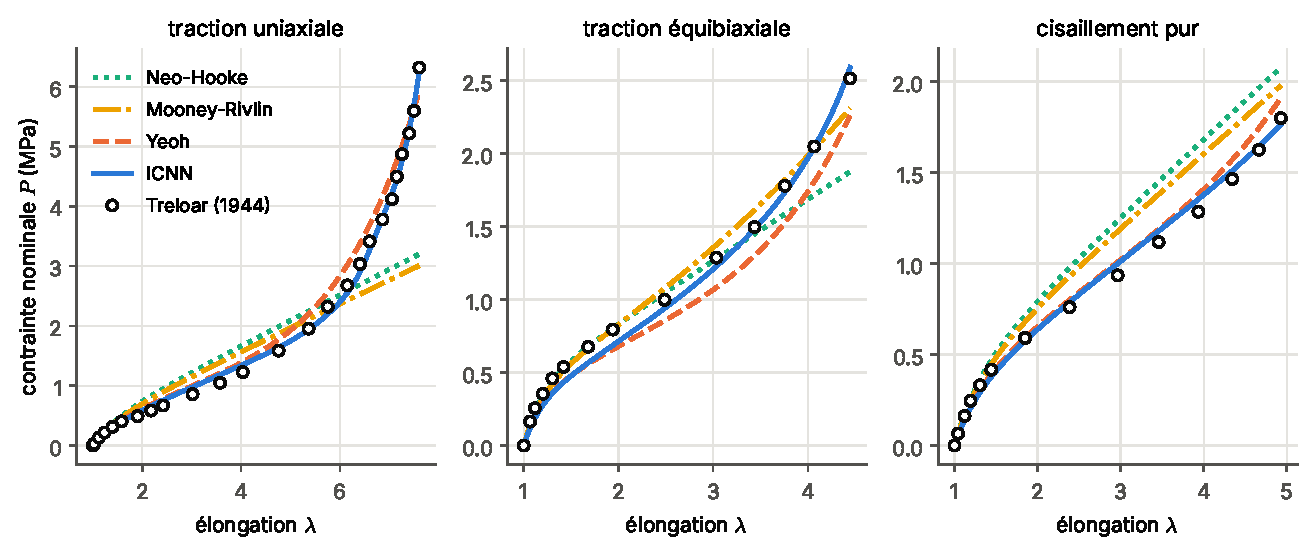
\includegraphics[width=\linewidth]{treloar_fit}
\caption{Identification sur les trois essais de Treloar.}\label{fig:treloar}
\end{figure}

\begin{figure}[h]
\centering
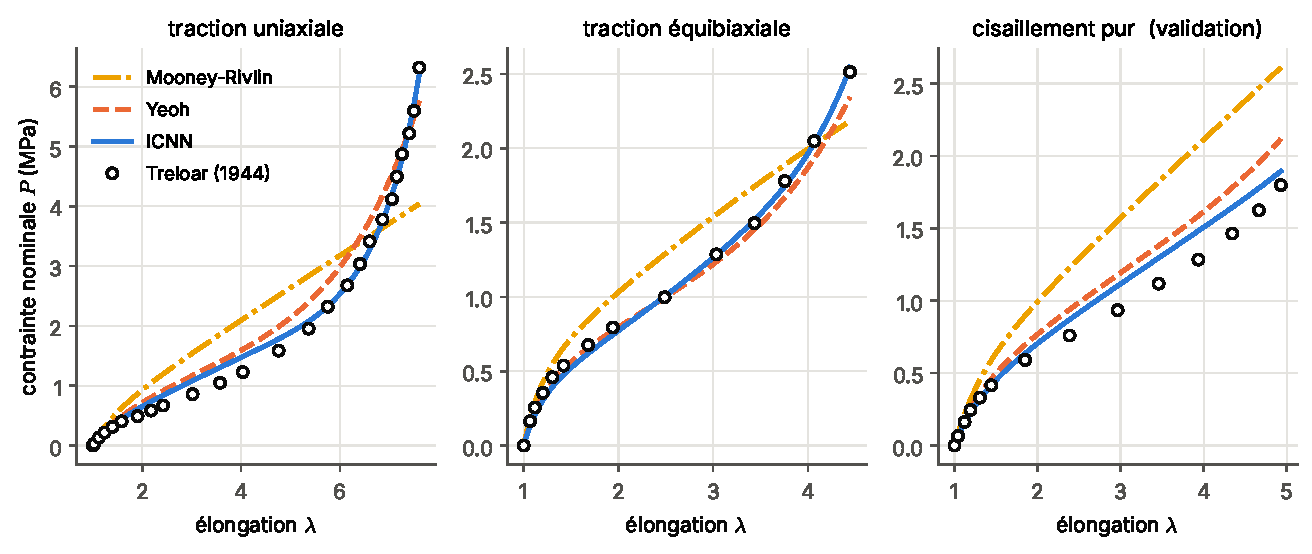
\includegraphics[width=\linewidth]{treloar_generalisation}
\caption{Identification sur UT et ET seulement. Le cisaillement pur (à droite) n'a pas servi à l'apprentissage.}\label{fig:treloar-gen}
\end{figure}

\begin{table}[h]
\centering
\begin{tabular}{l ccc ccc}
\toprule
 & \multicolumn{3}{c}{Apprentissage UT + ET + PS} & \multicolumn{3}{c}{Apprentissage UT + ET}\\
\cmidrule(lr){2-4}\cmidrule(lr){5-7}
Modèle & UT & ET & PS & UT & ET & PS (valid.)\\
\midrule
Neo-Hooke & $1{,}3\times10^{-1}$ & $2{,}8\times10^{-2}$ & $5{,}5\times10^{-2}$ & $8{,}0\times10^{-2}$ & $1{,}9\times10^{-2}$ & $2{,}6\times10^{-1}$\\
Mooney--Rivlin & $1{,}6\times10^{-1}$ & $3{,}7\times10^{-3}$ & $3{,}2\times10^{-2}$ & $7{,}5\times10^{-2}$ & $2{,}2\times10^{-2}$ & $3{,}0\times10^{-1}$\\
Yeoh & $5{,}3\times10^{-3}$ & $1{,}7\times10^{-2}$ & $4{,}7\times10^{-3}$ & $1{,}1\times10^{-2}$ & $3{,}1\times10^{-3}$ & $4{,}4\times10^{-2}$\\
ICNN & $\mathbf{8{,}4\times10^{-4}}$ & $\mathbf{3{,}6\times10^{-3}}$ & $\mathbf{1{,}7\times10^{-3}}$ & $\mathbf{1{,}7\times10^{-3}}$ & $\mathbf{1{,}1\times10^{-3}}$ & $\mathbf{1{,}4\times10^{-2}}$\\
\bottomrule
\end{tabular}
\caption{Erreur quadratique normalisée par essai (la racine donne l'ordre de l'erreur relative : $10^{-3}\leftrightarrow3\,\%$).}\label{tab:treloar}
\end{table}

\paragraph{Discussion.}
\begin{itemize}
  \item \textbf{Neo-Hooke et Mooney--Rivlin} ne reproduisent pas la remontée de la courbe uniaxiale au-delà de $\lambda\approx6$. Ce raidissement traduit l'extensibilité limitée des chaînes de polymère. Un potentiel linéaire en $I_1$ et $I_2$ ne peut pas le représenter : l'erreur relative en traction uniaxiale reste de 37 à 40\,\%.
  \item \textbf{Yeoh} capte la remontée grâce au terme cubique. Mais le coefficient identifié est $C_{20}<0$ : $\psi_1=C_{10}+2C_{20}x+3C_{30}x^2$ \emph{décroît} pour $x<7$, ce qui rend $\psi$ non convexe en $I_1$. La polyconvexité n'est plus garantie. C'est un défaut classique des polynômes identifiés sans contrainte.
  \item \textbf{L'ICNN} donne la meilleure précision sur les trois essais (erreur relative d'environ 3 à 6\,\%) \emph{et} garantit la polyconvexité. En validation sur le cisaillement pur, il prédit à environ 12\,\% près, contre 21\,\% pour Yeoh et 55\,\% pour Mooney--Rivlin. Les dérivées apprises sont physiquement lisibles : $\psi_1$ est presque constant jusqu'à $\lambda\approx5$ puis croît fortement (le raidissement), et $\psi_2$ est petit et positif (figure~\ref{fig:icnn-deriv}).
  \item \textbf{Limite.} La convexité interdit à $\psi_1$ de décroître. Or les données suggèrent une légère décroissance aux petites élongations, d'où la courbe légèrement au-dessus des points pour $2\le\lambda\le4$ en UT. Ce compromis est le prix de la garantie physique. Il peut être réduit avec $\psi_2$ et des invariants supplémentaires, comme dans les réseaux de type CANN~\cite{linka2021}.
\end{itemize}

\begin{figure}[h]
\centering
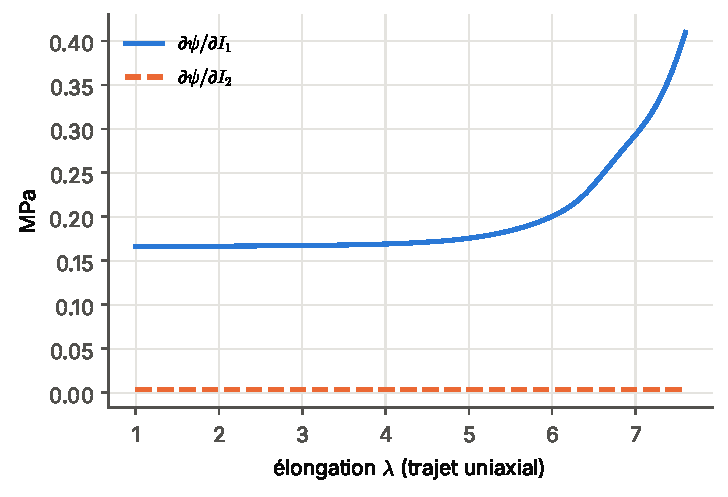
\includegraphics[width=0.55\linewidth]{treloar_icnn_derivatives}
\caption{Dérivées $\psi_1=\partial\psi/\partial I_1$ et $\psi_2=\partial\psi/\partial I_2$ de l'ICNN (scénario « tous ») le long du trajet uniaxial.}\label{fig:icnn-deriv}
\end{figure}

\section{Conclusion et perspectives}

\subsection{Ce qu'il faut retenir}

\begin{retenir}
\begin{enumerate}[nosep,leftmargin=*]
  \item \textbf{L'AD donne la tangente cohérente exacte.} Elle coïncide à $3\times10^{-16}$ près avec la formule de Simo--Hughes, et les différences finies plafonnent à $10^{-11}$. Écrire $\psi$ ou \code{integrate} suffit : la dérivation à la main devient un \emph{test}, et n'est plus une étape du développement.
  \item \textbf{Trois pièges, trois tests.} Un \code{if} est remplacé par \code{where}. Un \code{where} seul laisse passer des NaN en mode inverse, d'où le double \code{where}. La dérivation par rapport à une matrice $3\times3$ casse les symétries mineures, d'où le passage en Mandel.
  \item \textbf{Bien choisir le cas test.} Écrouissage linéaire et chargement proportionnel donnent une réponse affine par morceaux et un Newton qui converge en une itération. Pour \emph{voir} la convergence quadratique, il faut un écrouissage non linéaire (Voce) ou un chargement non proportionnel. On mesure alors un ordre de 2,01 contre 1,00 avec la tangente élastique, dont le taux de 0,130 se prédit par le spectre de $\mathbf{I}-\mathbf{K}_e^{-1}\mathbf{K}_t$.
  \item \textbf{Le noyau est limité par la mémoire.} JAX CPU est 3,5 à 4,5 fois plus rapide que NumPy grâce à la fusion. XLA laisse cependant un trafic 3,5 fois supérieur au minimum, qu'un noyau écrit à la main pourrait éliminer.
  \item \textbf{Le GPU n'a d'intérêt que si les données y résident.} Mesuré sur une RTX~2050 : avec données résidentes, il est 2 fois plus rapide que le CPU en FP64 et 4 fois en FP32. Avec transferts, il est 2 à 3 fois plus lent, car le bus PCIe prend près de 90\,\% du temps. Le FP64 de la carte vaut 1/52 de son FP32.
  \item \textbf{Un réseau peut être physique.} Un ICNN de 230 paramètres, polyconvexe par construction, reproduit les trois essais de Treloar à 3--6\,\% près et prédit le cisaillement pur non vu à 12\,\% près, contre 21\,\% pour le meilleur polynôme.
\end{enumerate}
\end{retenir}

\subsection{Perspectives}

\begin{itemize}[nosep]
  \item \textbf{Garder l'état sur le GPU} entre les itérations de Newton, et ne faire circuler que $\eps$ et $\sig$ : le plafond PCIe passerait de $10^7$ à $3\times10^7$ points/s en FP64, au-dessus du CPU (section~\ref{sec:gpu}). Utiliser aussi la mémoire hôte verrouillée pour accélérer le retour vers l'hôte.
  \item \textbf{Noyau fusionné} (Pallas ou CUDA) pour approcher le trafic minimal de 304~octets par point, et mesurer le gain par rapport à XLA.
  \item \textbf{Couplage avec un code EF}, par exemple avec la tangente exportée vers code\_aster ou FEniCSx, ou un assemblage complet en JAX pour garder l'état sur GPU.
  \item \textbf{Lois plus riches} : écrouissage cinématique non linéaire (Armstrong--Frederick, Chaboche), viscoplasticité, plasticité en grandes déformations. La dérivation implicite de la section~\ref{sec:implicit} s'étend telle quelle à un système non linéaire vectoriel.
  \item \textbf{Identification de paramètres} par gradient en mode inverse à travers \code{integrate}, sur une courbe d'essai complète. C'est le cas d'usage où le double \code{where} devient indispensable.
  \item \textbf{Précision mixte} : calculer la loi en FP32 et le résidu d'équilibre en FP64, en mesurant l'effet sur la convergence du Newton global.
\end{itemize}


\appendix
\section{Structure du dépôt et reproduction}\label{app:repo}

\begin{lstlisting}[language={}]
jax-j2-gauss/
|-- src/j2gauss/
|   |-- mandel.py        notation de Mandel, projecteurs
|   |-- j2.py            retour radial, version naive, custom_jvp
|   |-- tangent.py       tangentes AD / analytique / DF / elastique
|   |-- driver.py        pilotage mixte du point materiel
|   |-- j2_numpy.py      reference NumPy vectorisee
|   `-- hyperelastic.py  Neo-Hooke, essais homogenes, ICNN
|-- tests/               77 tests pytest
|-- scripts/             etudes : convergence, hysteresis, tangente, Treloar
|-- benchmarks/          bench_cpu_gpu.py, plot_bench.py, gpu_model.py, results/
|-- gpu/                 kit GPU : setup, diagnostic, benchmark, figures
|-- notebooks/           newton_convergence.ipynb, hysteresis.ipynb
|-- data/treloar.csv     donnees experimentales
|-- figures/             figures (PDF + PNG)
|-- results/             CSV des etudes
`-- report/              ce rapport (LaTeX)
\end{lstlisting}

Reproduction complète (environ 5~minutes sur CPU) :
\begin{lstlisting}[language=bash]
python3 -m venv .venv && source .venv/bin/activate
pip install -r requirements.txt
pytest -q                                   # 77 tests
cd scripts
python newton_convergence.py && python hysteresis.py && python tangent_accuracy.py
python fit_treloar.py && python make_notebooks.py
cd ..
python benchmarks/bench_cpu_gpu.py --nmax 6.5
python benchmarks/plot_bench.py benchmarks/results/bench_*.csv --name bench_cpu
python benchmarks/gpu_model.py
bash gpu/setup_gpu.sh                    # machine avec GPU NVIDIA
source .venv-gpu/bin/activate && bash gpu/run_all.sh
cd report && latexmk -xelatex rapport.tex
\end{lstlisting}

\section{Paramètres matériau}\label{app:params}

\begin{center}
\begin{tabular}{lcccccc}
\toprule
Jeu & $E$ (GPa) & $\nu$ & $\sigma_y$ (MPa) & $H$ (MPa) & $Q$ (MPa), $b$ & $C$ (MPa)\\
\midrule
linéaire (défaut) & 210 & 0,3 & 250 & 1000 & --- & ---\\
Voce & 210 & 0,3 & 250 & 1000 & 150, 50 & ---\\
Prager & 210 & 0,3 & 250 & 0 & --- & 8000\\
Voce + Prager (benchmarks) & 210 & 0,3 & 250 & 1000 & 150, 50 & 5000\\
\bottomrule
\end{tabular}
\end{center}
Les données du benchmark sont aléatoires : $\eps\sim\mathcal{N}(0,(3\times10^{-3})^2)$, $\epsp$ et $\X$ déviatoriques de petite amplitude, $p\sim\mathcal{U}(0;0{,}02)$.


\begin{thebibliography}{99}\small
\bibitem{simo1998} J.~C. Simo, T.~J.~R. Hughes. \emph{Computational Inelasticity}. Springer, 1998.
\bibitem{desouza2008} E.~A. de Souza Neto, D.~Perić, D.~R.~J. Owen. \emph{Computational Methods for Plasticity: Theory and Applications}. Wiley, 2008.
\bibitem{griewank2008} A.~Griewank, A.~Walther. \emph{Evaluating Derivatives: Principles and Techniques of Algorithmic Differentiation}, 2\textsuperscript{e} éd. SIAM, 2008.
\bibitem{jax2018} J.~Bradbury \emph{et al.} JAX: composable transformations of Python+NumPy programs. \url{https://github.com/jax-ml/jax}, 2018.
\bibitem{blondel2022} M.~Blondel \emph{et al.} Efficient and modular implicit differentiation. \emph{NeurIPS}, 2022.
\bibitem{williams2009} S.~Williams, A.~Waterman, D.~Patterson. Roofline: an insightful visual performance model for multicore architectures. \emph{Communications of the ACM}, 52(4):65--76, 2009.
\bibitem{voce1948} E.~Voce. The relationship between stress and strain for homogeneous deformation. \emph{Journal of the Institute of Metals}, 74:537--562, 1948.
\bibitem{prager1956} W.~Prager. A new method of analyzing stresses and strains in work-hardening plastic solids. \emph{Journal of Applied Mechanics}, 23:493--496, 1956.
\bibitem{treloar1944} L.~R.~G. Treloar. Stress-strain data for vulcanised rubber under various types of deformation. \emph{Transactions of the Faraday Society}, 40:59--70, 1944.
\bibitem{ball1977} J.~M. Ball. Convexity conditions and existence theorems in nonlinear elasticity. \emph{Archive for Rational Mechanics and Analysis}, 63:337--403, 1977.
\bibitem{amos2017} B.~Amos, L.~Xu, J.~Z. Kolter. Input convex neural networks. \emph{ICML}, 2017.
\bibitem{linka2021} K.~Linka \emph{et al.} Constitutive artificial neural networks: a fast and general approach to predictive data-driven constitutive modeling by deep learning. \emph{Journal of Computational Physics}, 429:110010, 2021.
\bibitem{yeoh1993} O.~H. Yeoh. Some forms of the strain energy function for rubber. \emph{Rubber Chemistry and Technology}, 66(5):754--771, 1993.
\bibitem{helfer2015} T.~Helfer \emph{et al.} Introducing the open-source MFront code generator. \emph{Computers \& Mathematics with Applications}, 70(5):994--1023, 2015.
\end{thebibliography}


\end{document}
